\chapter{Executing Large Scale Workflow Ensembles in Public Clouds}
\label{chapter:dewe_v2}

\section{Introduction}
\label{sec:intro}

Many applications in science and engineering are increasingly formed as workflows with many precedence-constrained jobs, e.g., Montage \cite{montage, web:montage}, LIGO \cite{ligo}, and CyberShake \cite{cybershake}. Scientists need to run these workflows with different parameters repeatedly, or use a combination of different workflows to achieve an ultimate goal. We use the term \textbf{workflow ensemble} to represent an entire scientific analysis as a set of interrelated but independent workflow applications. In modern scientific computing applications, a single scientific workflow often becomes very large in terms of the number of constituting jobs and input data size, which is already a challenge in terms of resource provisioning and scheduling. The situation is further complicated by the number of interrelated but independent workflows in a workflow ensemble. Thus, the efficient execution of a workflow ensemble with multiple workflows is of great practical importance.

Most researchers in the scientific workflow community use existing workflow management systems that were designed with grid as the target execution environment. In a grid environment, the computing resources are considered as heterogeneous. It is necessary to schedule critical jobs to worker nodes with more processing power, and to avoid large data transfer over connections with small bandwidth. In public clouds, a homogeneous environment can be created by launching instances with the same instance type in the same availability zone. This brings new opportunities in optimizing execution coordination, which was not considered in existing workflow management systems. From a cost perspective, most service providers charge computing resources in an hourly manner, where partial hour usage is charged as a full hour. For example, a particular workflow takes 61 minutes to execute on a 10-node cluster, but can be completed in 59 minutes on a 11-node cluster. The cost to run the workflow on a 10-node cluster is 20 instance hours, but would be only 11 instance hours on a 11-node cluster. For large scale workflow ensembles, it is critical that the execution can be completed within both cost and deadline constrains. There have been some previous studies on these two aspects. However, existing literature only provides small scale results or uses simulations instead of real scientific applications.

\begin{figure}[!t]
	\centering
	\hspace{-10pt}
	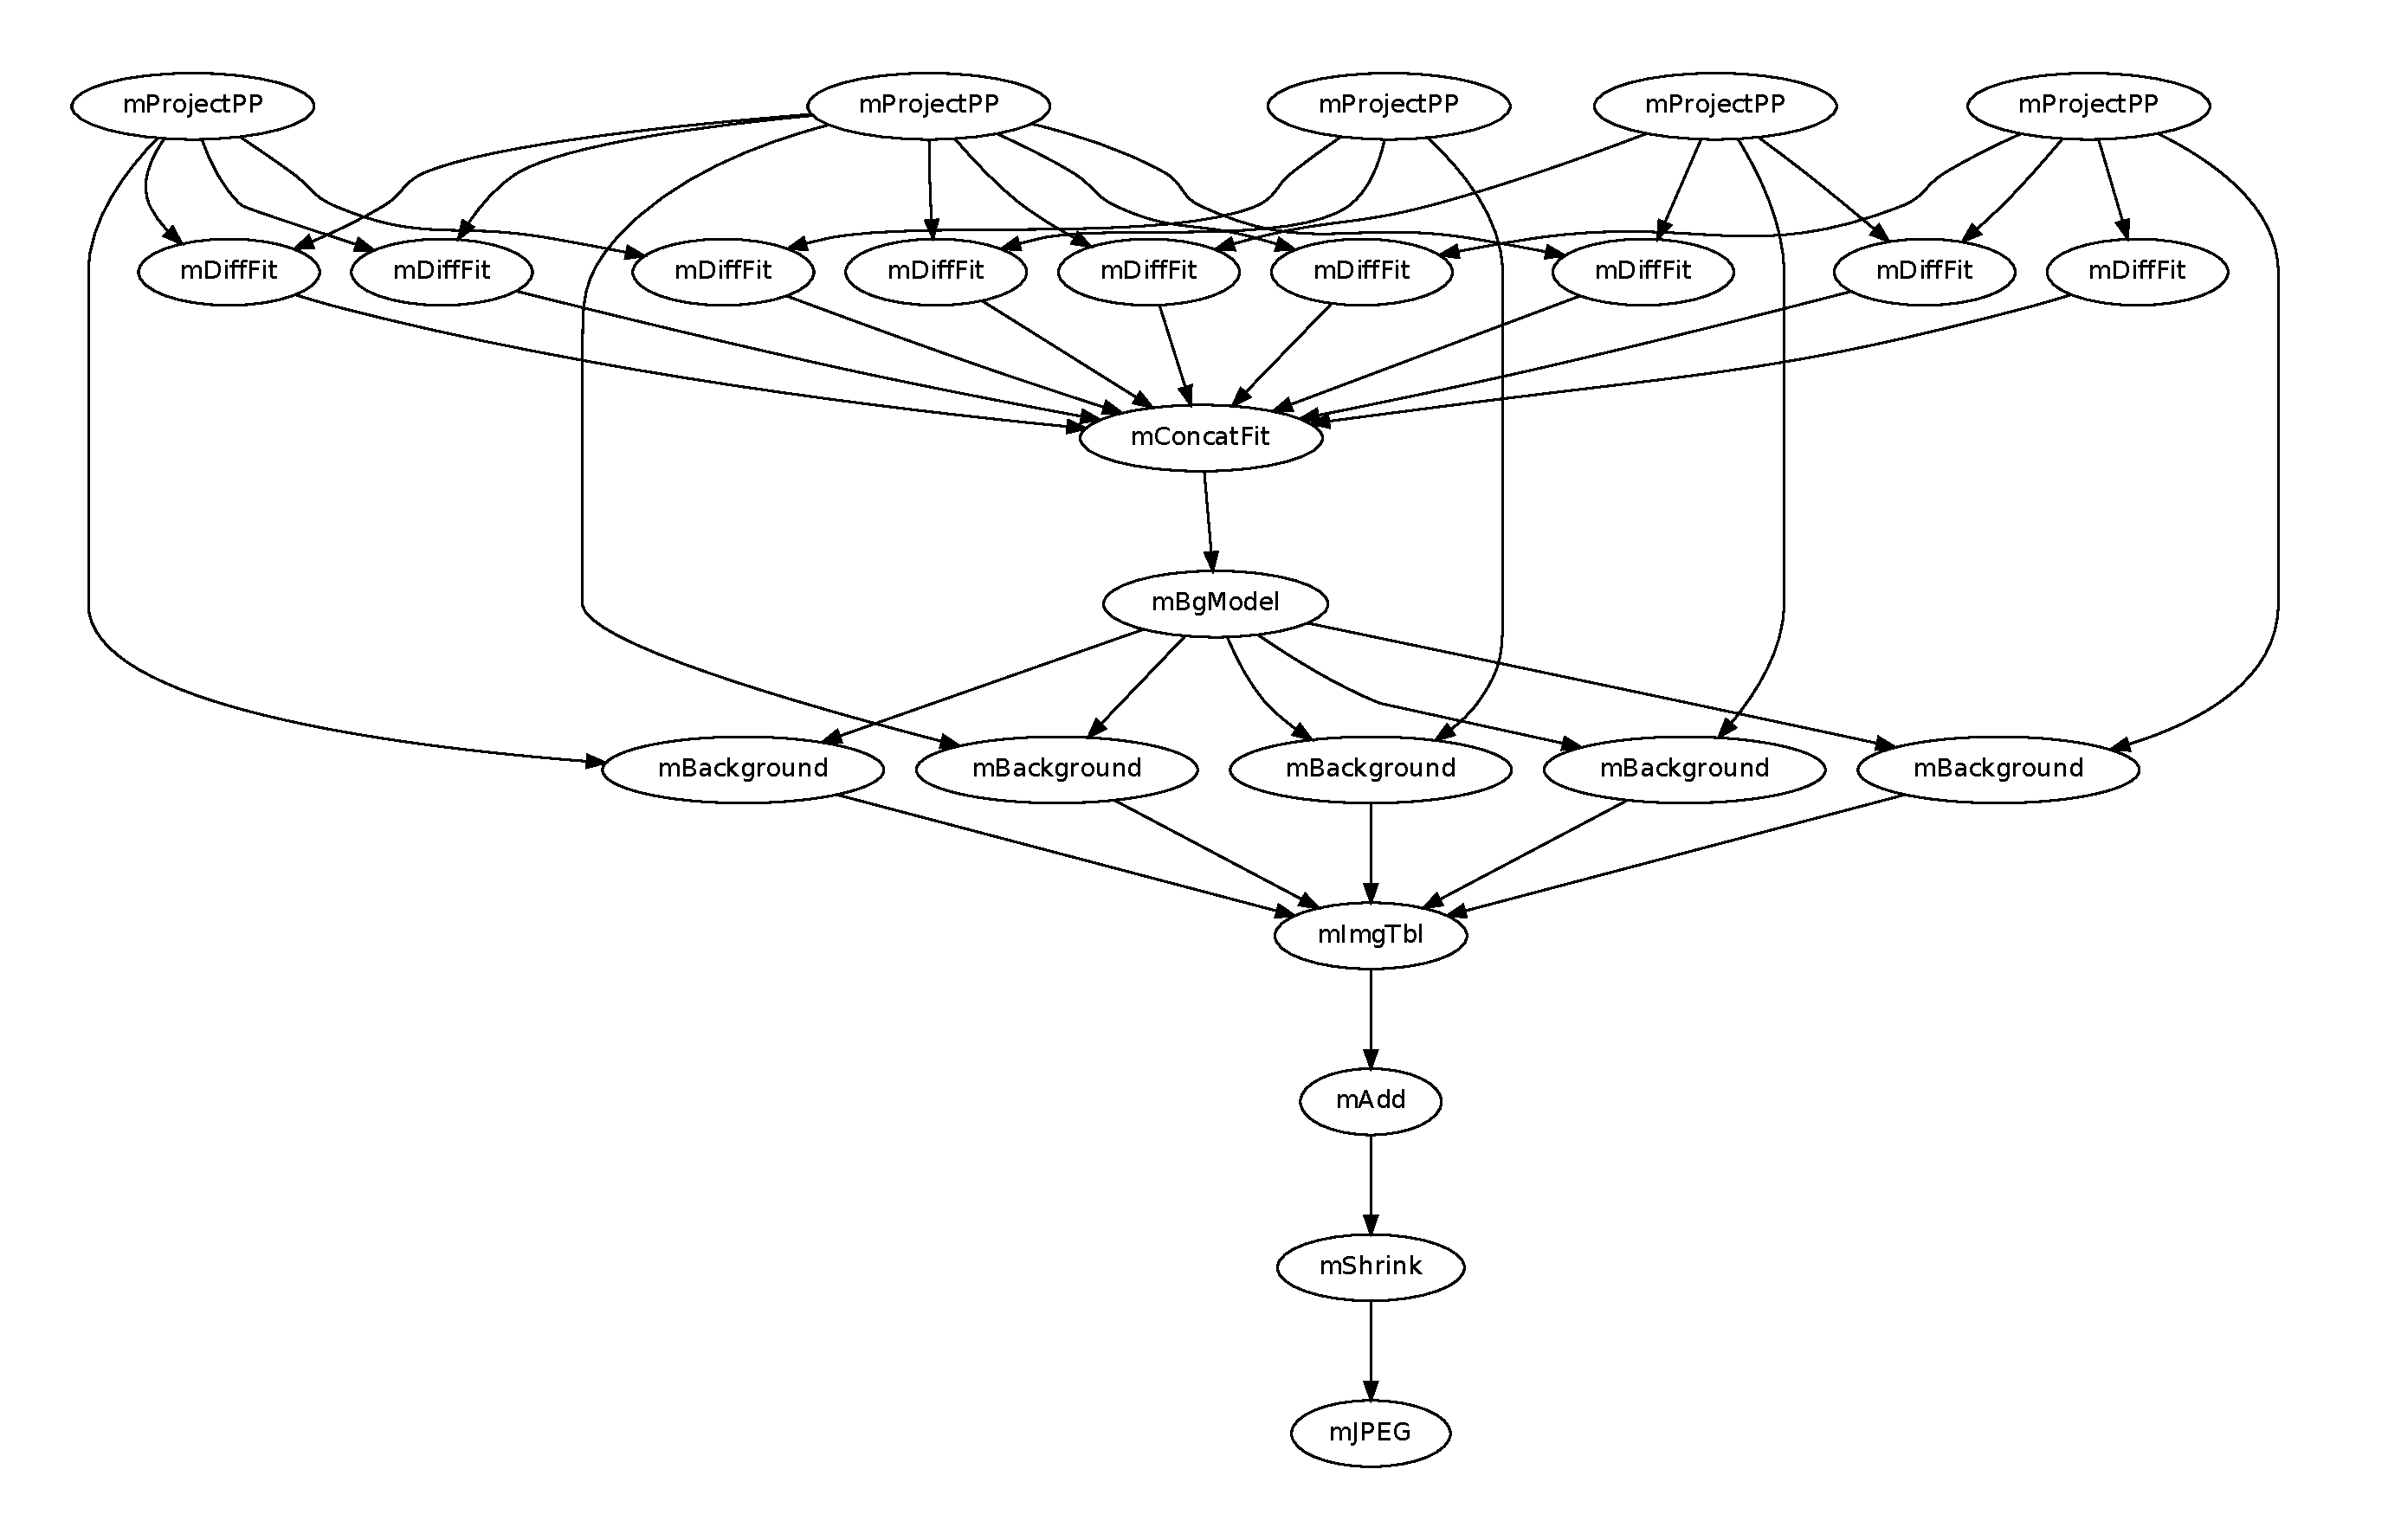
\includegraphics[width=9.7cm, height=7cm]{montage}
    \caption{The structure of the Montage workflow.}
    \vspace{-10pt}
	\label{fig:montage}
\end{figure}

\begin{figure*}[ht]
\centering
\fbox{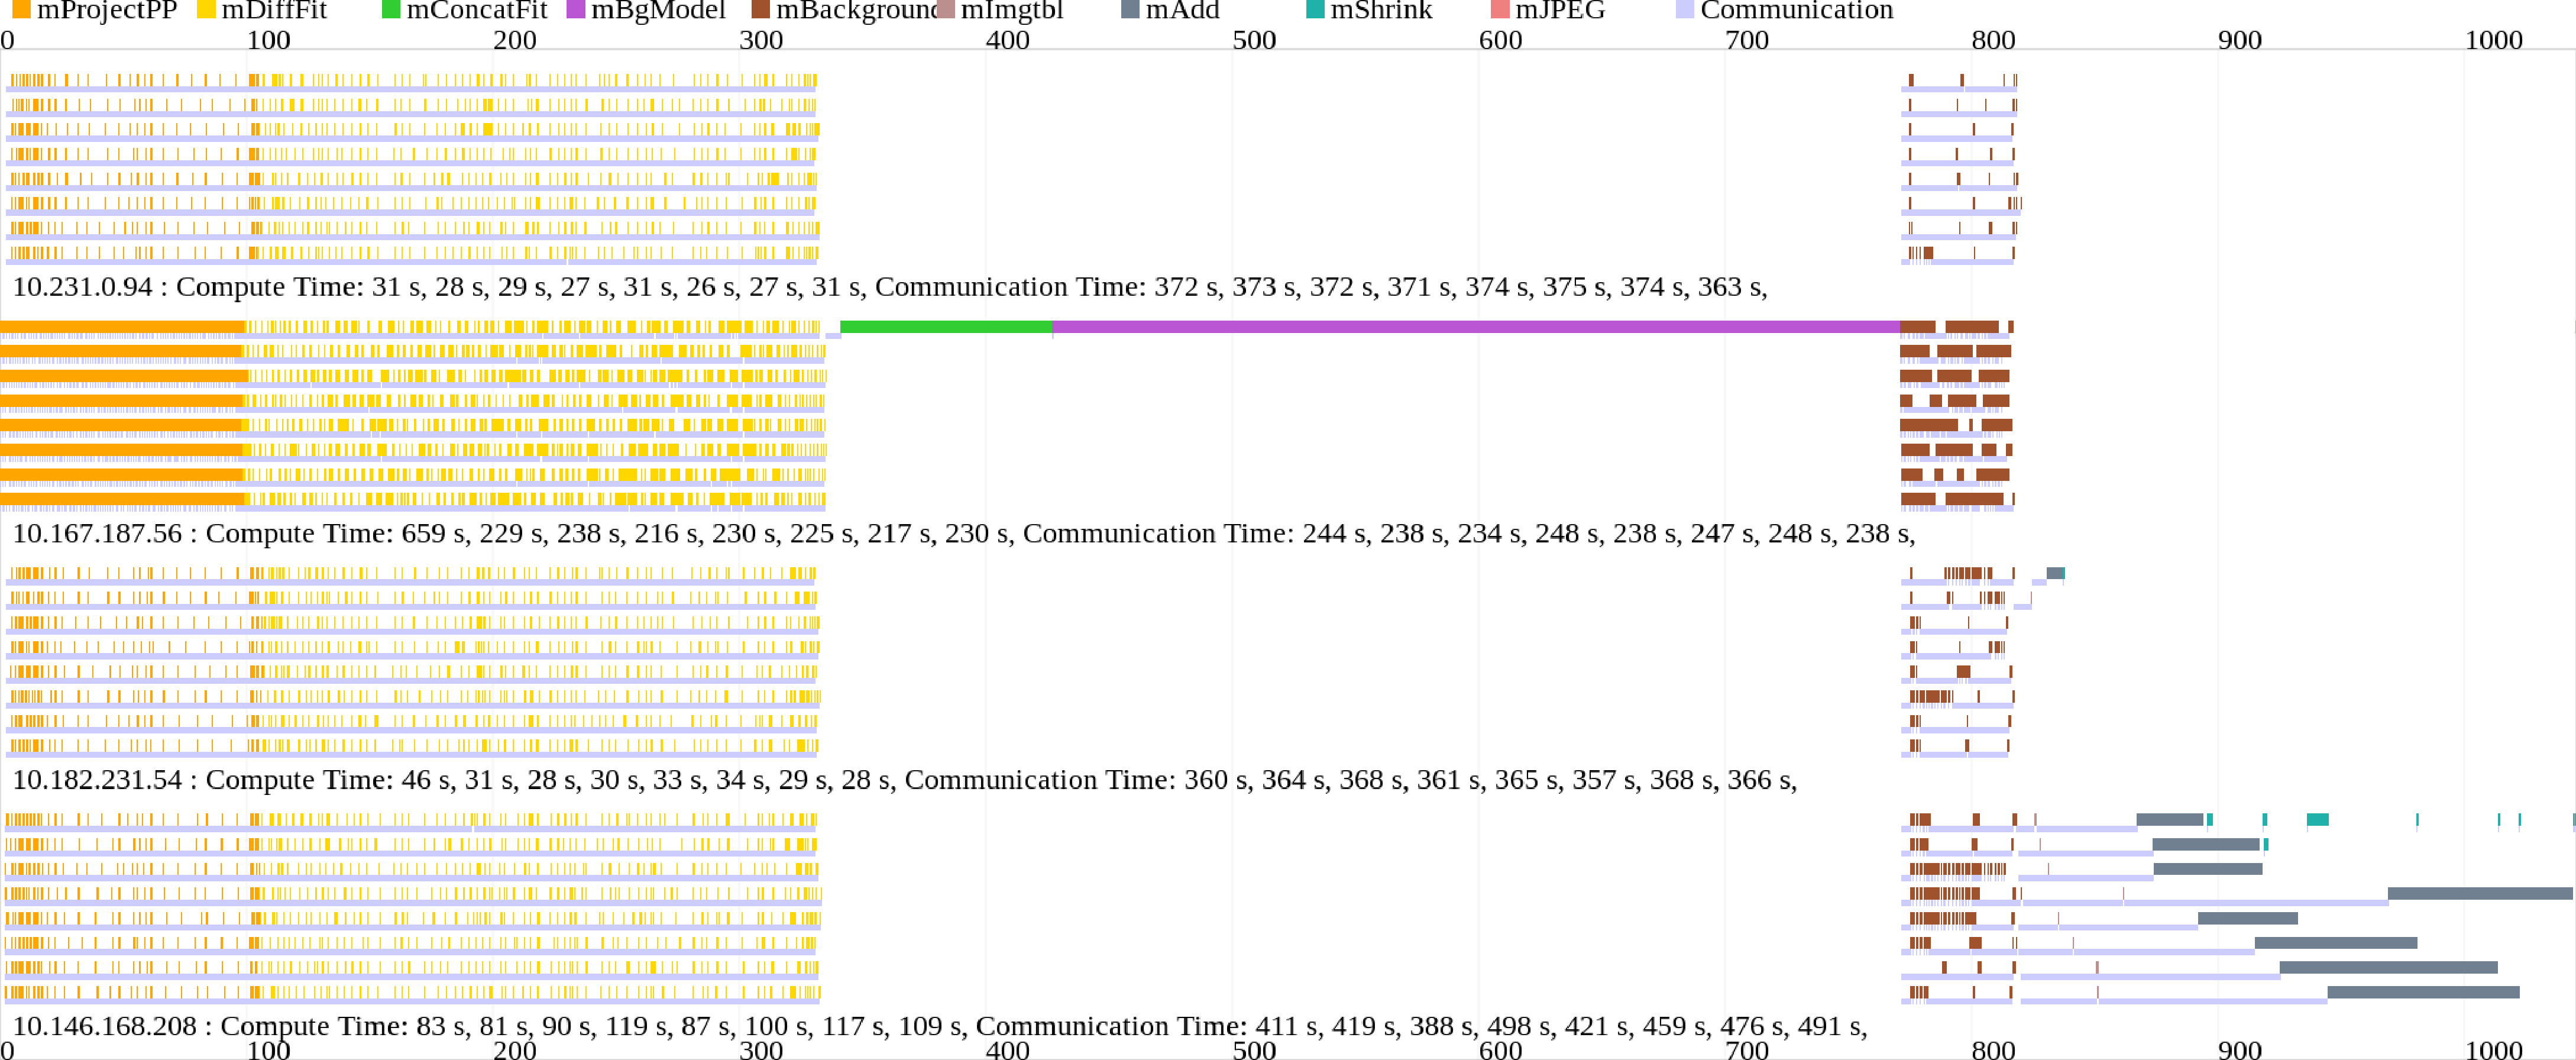
\includegraphics[width=16cm]{montage_visualization}}
\caption{Detailed visualization of a 6.0 degree Montage workflow running 4 m3.2xlarge instaces using DEWE v1. Each worker node has 8 vCPU, 30 GB of memory, and 2 x 80 GB SSD storage. The horizontal axis represents time in seconds, while the vertical axis represents vCPU slots in the cluster. Each vCPU is represented by two horizontal bars, with job execution activities on the first horizontal bar and data staging activities on the second horizontal bar. For each worker node, the graph shows the IP address of the worker node, the time spent on job execution (compute time) and the time spent on data staging (communication time) for each vCPU slot. As shown in the graph, the Montage has a clear three-stage pattern, with significant resource utilization in the second and third stage.}
\label{fig:montage_visualization}
\end{figure*}

In this chapter, we choose Montage as a representative example of large scale scientific workflows for our case study due to the following reasons:  (1) there are a large number of small jobs that can run in parallel, (2) scientists in astronomy do have the need to execute Montage workflow ensembles; for example, a set of small image mosaics are needed to produce a large image mosaic (the Galactic Plane workflow ensemble \cite{deelman2013hosted} consists of 17 workflows, each of which contains 900 sub-workflows), (3) Montage workflows are data-intensive, and (4) The Montage source code and data is available to the general public (i.e., open source). (1) is closely related to execution coordination, (2) presents challenges in resource provisioning, and (3) is closely related to data staging. Therefore, Montage is an ideal example that enables us to study these three challenges in executing large scale workflow ensembles in public clouds.

Montage is an astronomical image mosaic engine that assembles individual images of the sky into a mosaic. A 6.0 degree Montage workflow creates a 6-by-6 degree square mosaic centered at a particular region of the sky (e.g., M16). The number of jobs and input data files increases with the number of degrees of the mosaic. A 6.0 degree Montage workflow contains 8,586 jobs, 1,444 input files with a total size of 4.0 GB, and 22,850 intermediate files with a total size of 35 GB. In practice, a set of smaller image mosaics are needed to produce a large image mosaic, where each smaller image mosaic is generated by a Montage workflow. For example, the Galaetic Plane workflow ensemble \cite{deelman2013hosted} consists of 17 workflows, each of which further contains 900 sub-workflows. 


Figure \ref{fig:montage} describes the structure of the Montage workflow. The progress of the workflow has a three-stage pattern. During the first stage, a large number of mProjectPP jobs run in parallel, followed by a large number of mDiffFit jobs running in parallel. During the second stage, two jobs mConcatFit and mBgModel run one after another, during which no other jobs are eligible to run. In this paper, we consider mConcatFit and mBgModel as blocking jobs because they block the execution of other jobs. During the third stage, a large number of mBackground jobs run in parallel, followed by a small number of mImgTbl, mAdd, mShrink, and mJPEG jobs.

As shown in Figure  \ref{fig:montage_visualization}, the mProjectPP, mDiffFit and mBackground jobs are small jobs with very short execution time within the range of a few seconds. However, they consume and produce a large number of intermediate data files. Staging these intermediate data files between worker nodes causes significant communication cost. Considering the large number of such jobs, it is desirable to have more worker nodes to speed up the execution. However, the communication costs increases when the number of worker nodes increases, resulting in clustering performance degradation. Furthermore, the execution time of the second stage is approximately 40\% of the makespan. During this stage, among all the available computing resources only one CPU core is being utilized. When the cluster is larger, more computing resources are being wasted during this stage. In a Montage workflow ensemble, resource under-utilization can be worse due to the lack of coordination between individual sub-workflows. Therefore, the Montage workflow ensemble represents a scheduling dilemma requiring trade-offs between cost and performance. 

In this chapter, we address two main challenges in realizing benefits of using public clouds when executing large-scale workflow ensembles with both deadline and cost constrains: (1) execution coordination, and (2) resource provisioning. To this end, we develop DEWE v2 \footnote{The source code is available from \url{https://github.com/qyjohn/DEWE.v2}.}, a major overhaul of our preliminary version of DEWE \cite{dewev1}. DEWE v2 is a pulling-based workflow execution system that is capable of executing large scale scientific workflow ensembles in public clouds. Using DEWE v2, we address the above-mentioned challenges in executing large-scale workflow ensembles in public clouds. The specific contributions of this paper are:


\begin{itemize}
  \item We demonstrate that the pulling approach has better performance over the scheduling approach in executing large scale scientific workflow ensembles in public clouds. 
  \item We demonstrate that incremental job submission can effective shape the resource utilization pattern, thus achieve better resource utilization than batch job submission. 
  \item We propose a two-step strategy to provision computing resources in public clouds for executing large scale scientific workflow ensembles to meet both cost and deadline constraints. 
\end{itemize}

We have extensively evaluated DEWE v2 using Montage workflow ensembles with varying sizes and different configurations of EC2 clusters. In particularly, our large-scale experiments were conducted using up to 200 6.0 degree Montage workflows containing over 1.7M jobs and dealing with approximately 7 TB of data; and, four Amazon EC2 clusters with different instance types (\emph{c3.8xlarge, r3.8xlarge and i2.8xlarge}, which are the largest instances in their instance families) were set up consisting of up to 1,280 vCPUs. 

The rest of this chapter is organized as follows. In Section \ref{v2_sec:dewe_v2_design}, we describe the design philosophy, system architecture, and the implementation of DEWE v2. In Section \ref{v2_sec:dewe_v2_performance}, we evaluate the performance of DEWE v2, using Pegasus as a comparison. We also compare the the efficiency of batch submission and incremental submission, as will as the robustness of DEWE v2. In Section \ref{v2_sec:provision}, we propose a two-step strategy to provision computing resources in public clouds for executing large scale scientific workflow ensembles with both cost and deadline constraints. We demonstrate the effectiveness of the proposed resource provisioning strategy with its incorporation into DEWE v2. 


\section{Design and Implementation of DEWE v2}
\label{v2_sec:dewe_v2_design}

DEWE v2 is an improved version of DEWE, a lightweight framework for distributed elastic workflow execution developed at the University of Sydney. In subsequent sections, we call the original version DEWE v1.  DEWE v2 shares some fundamental design concepts with DEWE v1; hence the name. With DEWE v1, researchers can only execute one workflow at a time. DEWE v2 is capable of executing a large number of workflows in parallel, hence the ability to execute large-scale workflow ensembles. DEWE v1 was developed in Python, and DEWE v2 was developed in Java to reduce third-party package dependencies. 

In this section, we describe the design philosophy, system architecture, as well as the implementation of DEWE v2. 


\subsection{Design Philosophy}
\label{sec:subsec:design_philosophy}


In general, there are two approaches to design and implement a workflow management system. The first approach emphasizes scheduling where the master node maintains the state of all participating worker nodes, assigns jobs to worker nodes using various resource scheduling algorithms, as well as stages necessary data files to the worker nodes for job execution. The second approach emphasizes a stateless design where the master node publishes all pending jobs to a queue, and a number of un-managed worker nodes pull the job queue and compete for jobs to execute. Most existing workflow management systems adopt the scheduling approach, including Condor DAGMan, Pegasus, and Kepler. 

In a grid environment, the computing resources are considered as heterogeneous. It is necessary to schedule critical jobs to worker nodes with more processing power, and to avoid large data transfer over connections with small bandwidth. Furthermore, data transfer between worker nodes is usually accomplish with file transfer tools such as FTP, SFTP, GridFTP, or SCP. In the workflow community, the cost to stage the output of one job to the node that will run the second job is defined as communication cost. An important assumption with the scheduling approach is the communication cost is none-zero value when both jobs are running on two different nodes, but becomes zero when the two jobs are running on the same node because no data transfer is needed. Therefore, a good scheduling algorithm should always try to minimize data transfers. With the scheduling approach, the scheduling overhead can be overcome by utilizing the computing resources in a more efficient way, resulting in shorter makespan. 

With Amazon EC2, a homogeneous environment can be achieved by launching all the worker nodes with the same instance type in the same placement group. For critical jobs, the computation cost remains the same regardless of the worker node they run on. Furthermore, data transfer between worker nodes can be replaced with a shared file system such as NFS. With a large scale workflow ensemble, the number and size of the input files overwhelm the memory available on the worker nodes. The result is the communication cost becomes the time needed to read the input files from the shared file system, which is the same regardless of the worker node. In this case, the pulling approach has advantages over the scheduling approach because it avoids the scheduling overhead.


\subsection{System Architecture}
\label{sec:subsec:system_architecture}

\begin{figure}[!t]
	\centering
	\hspace{-5pt}
	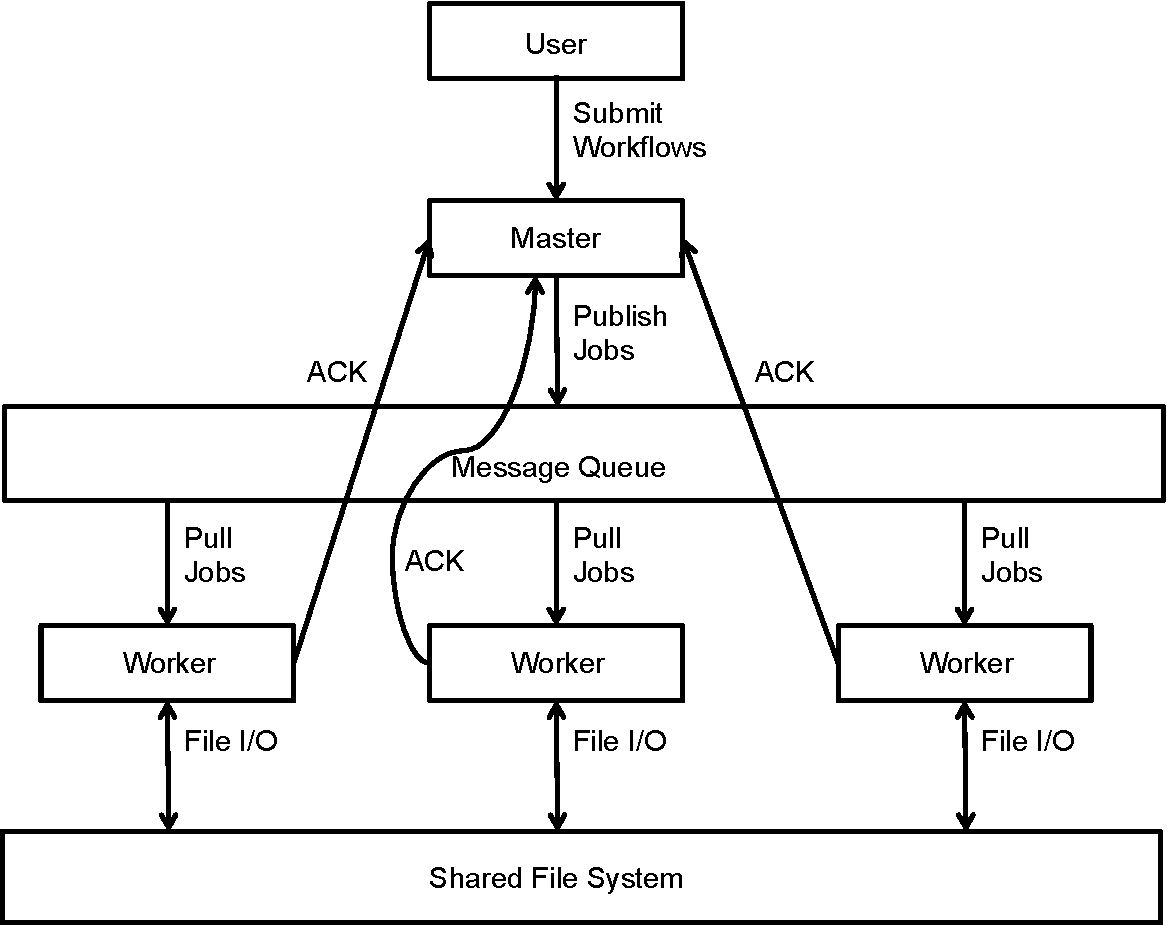
\includegraphics[width=7cm]{dewe_v2_architecture}
    \vspace{5pt}
	\caption{The architecture of DEWE v2.}
	\label{fig:dewe_v2_architecture}
\end{figure}


Both DEWE v1 and DEWE v2 are pulling based workflow execution engines, with a master node managing a message queue and multiple worker nodes pulling the message queue for jobs to execute. With DEWE v1, the master node also manages the input and output files. When a worker node pulls a job for execution, it queries the master node for the location of the input files, transfers the input files from the worker nodes that have/produce those files, executes the job and reports the results back to the master node. DEWE v2 removes this scheduling layer by utilizing a POSIX-compliant shared file system, which significantly simplify the architecture design. 



Figure \ref{fig:dewe_v2_architecture} shows the architecture design of DEWE v2. The system includes a master daemon, a worker daemon, and a workflow submission application. In a cluster environment, one of the nodes runs the master demon, which can optionally run the worker daemon at the same time. All other nodes run the worker daemon. Using the workflow submission application, scientists can submit workflows to the master daemon from any nodes at any time. 

The master daemon only manages the progress of the workflow, and publishes jobs that are eligible to run to a message queue. It has no knowledge about the worker nodes, but assumes that the worker nodes are homogeneous in terms of computing capability and communication bandwidth. 

On the basis of ``first come, first served", the worker nodes actively pull the message queue for jobs to execute. When the job is successfully executed, the worker node sends an acknowledge message to the master daemon. Based on the acknowledge messages from the worker nodes, the master daemon publishes new jobs that are eligible to run to the message queue.

A POSIX-compliant shared file system is used to facilitate the data sharing between worker nodes. When an output file is generated by a job on a worker node, it is immediately accessible from other worker nodes and can be used as inputs files for other jobs. This shared file system can be provided by either a centralized storage server (such as a NAS device) or a distributed storage system (such as GlusterFS). We assume that all worker nodes have equal access to the shared file system. A workflow is encapsulated in a folder on the shared file system, including the DAG file, the executable binaries, as well as the input and output files. 

To increase the robustness of the system, a timeout mechanism is added to the DAG management module in the master daemon. A job can have a user-defined timeout value or a system-wide default timeout value. If a job has been checked out from the message queue for execution but the corresponding acknowledgment is not received by the master daemon within the timeout setting, the master daemon publishes the job to the message queue again. With this timeout approach, any worker node can fail at any time and the failed jobs will be automatically resubmitted to the message queue for execution by other worker nodes when the timeout occurs.

The master daemon is capable of managing multiple workflows concurrently. When precedence dependencies are met, jobs in different workflows are published to the same message queue for execution. Therefore, multiple workflows can be executed in parallel on the same cluster. 

As we can see, DEWE v2 significantly simplifies the workflow execution process. There is no scheduling at any stage during the execution of the workflow. The stateless design of the worker node allows the cluster to scale in or scale out according to the actual workload requirements. 



\subsection{Implementation of the Master Daemon}
\label{sec:subsec:master_daemon}

At the core of DEWE v2 is a message queue system based on RabbitMQ. We use three separate topics in the message queue for workflow submission, job dispatching, and job acknowledgment. When the workflow submission application submits a workflow, meta data about the workflow (the name of the workflow, as well as the path to the related folder on the shared file system) is published to the workflow submission topic. The master daemon pulls meta data about the workflow from the workflow submission topic, then parses the DAG file and stores the job dependencies information into a data structure. If a job has no pending dependency precedence requirements, the master daemon publishes meta data about the job (the location of the binary executable with input and output parameters) to the job dispatching topic.

When a job is checked out by a worker node for execution, the worker nodes sends a message to the job acknowledgment topic indicating the job is now running. When a job is successfully executed on a worker node, the worker node sends another message to the job acknowledgment topic indicating the job is now completed. The master daemon pulls the job acknowledgment topic for such messages. If the message indicates a job is running, the master daemon marks the job as "running" so that the job is no longer visible to other worker nodes. If the message indicates a job is completed, the master daemon marks the job as "completed" and updates the status of all pending jobs that depend on the completed job. When a job has no pending precedence requirements it becomes eligible to run. Then the master daemon publishes meta data about jobs that are eligible to run to the job dispatching topic, where they are pulled by the worker nodes for execution.

The master daemon periodically examines the execution status of all "running" jobs. If a job is checked out by a worker node for execution but the corresponding acknowledgment indicating the job is completed is not received within its timeout setting, a timeout event is triggered. The master daemon then resubmits meta data about the job to the job dispatching topic so that other worker nodes can execute the job again.


\subsection{Implementation of the Worker Daemon}
\label{sec:subsec:worker_daemon}

The worker daemon has a stateless design. The only knowledge it has about the whole workflow execution system is the address of the message queue. It has no knowledge about the master node, other worker nodes in the system, or the jobs that have been executed on the worker node itself. It reads input files from, and writes output files to, the shared file system, just like using a local file system. Such a stateless design allows the cluster to scale in or scale out according to the actual workload requirements. 

The worker daemon pulls the job dispatching topic for jobs to execute. Upon receiving a job from the message queue, the worker daemon sends a message to the job acknowledgment topic indicating the job is now running. A separate thread is launched by the worker daemon to handle each individual job. Upon completion of the job, the worker daemon sends another message to the job acknowledgment topic indicating the job is now completed. The thread associated with a job is terminated when the job is completed. 

To avoid resource competition among concurrently running jobs, we put an upper limit on the number of concurrent job execution threads. The worker daemon stops pulling the job dispatching topic when the number of concurrent job execution threads equals to the number of CPUs available on the worker node. However, the worker daemon does not bind a job to a particular CPU. If a job is implemented in a way that can leverage multiple CPUs (for example,  OpenMP) the desired behavior is preserved. This feature can significant speed up the execution of a workflow when the blocking jobs (such as mConcatFit and mBgModel) are implemented as parallel code. 

\subsection{Implementation of the Workflow Submission Application}
\label{sec:subsec:submission_application}

The workflow submission application accepts two parameters from the user - the name of the workflow, and the path to the related folder on the shared file system. The workflow submission application publishes this information to the workflow submission topic in the message queue system, where it is checked out by the master daemon for further processing. 




\section{Experiment Environment}
\label{v2_sec:setup}

\subsection{Selection of EC2 Instances}
\label{sec:subsec:ec2_selection}


\begin{table}[t!]
\caption{EC2 Instance Types}
\label{tbl:instance_type}
\centering
\begin{tabular}{|p{2.5cm}|p{1.5cm}|p{1.5cm}|p{1.5cm}|p{1.5cm}|p{2.5cm}|}
\hline
Model & vCPU & Memory (GB) & Storage (GB) & Network (Gbps) & Hourly Price  (USD)\\ \hline
c3.8xlarge & 32 & 60  & 2 x 320 & 10 & 1.68\\ \hline
r3.8xlarge & 32 & 244 & 2 x 320 & 10 & 2.80\\ \hline
i2.8xlarge & 32 & 244 & 8 x 800 & 10 & 6.82\\ \hline
\end{tabular}
\end{table}



\begin{table}[t!]
\caption{Disk I/O Capacity of EC2 Instance Types}
\label{tbl:instance_disk_io}
\centering
\begin{tabular}{|p{2.5cm}|p{2.5cm}|p{2.5cm}|p{2.5cm}|p{2.5cm}|}
\hline
Model & Sequential Read (MB/s) & Sequential Write (MB/s) & Random Read (MB/s)& Random Write (MB/s)\\ \hline
c3.8xlarge & 250 & 800  & 400 & 600 \\ \hline
r3.8xlarge & 350 & 1000 & 700 & 800 \\ \hline
i2.8xlarge & 2200 & 3800 & 1800 & 3600 \\ \hline
\end{tabular}
\end{table}



Amazon Web Services (AWS) are widely recognized as examples of public cloud services. Over the past years, the market witnessed a trend in developing new applications on AWS, or migrating existing applications to AWS. In this paper, all the experiments are carried out on AWS Elastic Computer Cloud (EC2) in its us-east-1 (N. Virginia) region. AWS EC2 provides a wide range of instance types for different use cases. Different instance types have different combinations of vCPU, memory, storage, and networking capacity. We use the c3.8xlarge, r3.8xlarge, and i2.8xlarge instance types for our experiments. With AWS EC2, c3.8xlarge is the largest instance type for compute intensive applications, r3.8xlarge is the largest instance type for memory intensive applications, and i2.8xlarge is the largest instance type for storage intensive applications. Table \ref{tbl:instance_type} lists the specifications of the selected instance types. Apart from the properties listed in Table \ref{tbl:instance_type}, c3.8xlarge instance type uses Intel Xeon E5-2680 v2 (Ivy Bridge) processors, while r3.8xlarge and i2.8xlarge instance types use Intel Xeon E5-2670 v2 (Ivy Bridge) processors.  

On all of the selected instance types, the storage devices are SSD-backed instance store volumes (storage from disks that are physically attached to the host computer). To achieve the best disk I/O performance, we combine all the instance store volumes available on the instance using redundant array of independent disks (RAID) technology in a RAID 0 configuration. All the workflow related disk I/O operations are configured to occur on the RAID device. The file system being used on all worker nodes is ext4.

\subsection{Benchmark of EC2 Instances}
\label{sec:subsec:ec2_benchmark}

\begin{figure*}[t!]
\centering
\vspace{-10pt}
 \subfloat[CPU Benchmark]{ 
    \label{fig:subfig:benchmark_cpu}  
    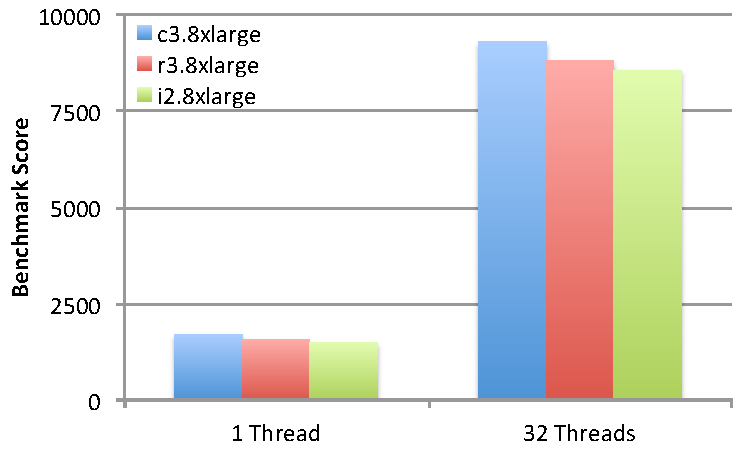
\includegraphics[width=6cm]{benchmark_cpu}} 
 \hspace{5pt}
 \subfloat[Memory Benchmark]{ 
    \label{fig:subfig:benchmark_mem}  
    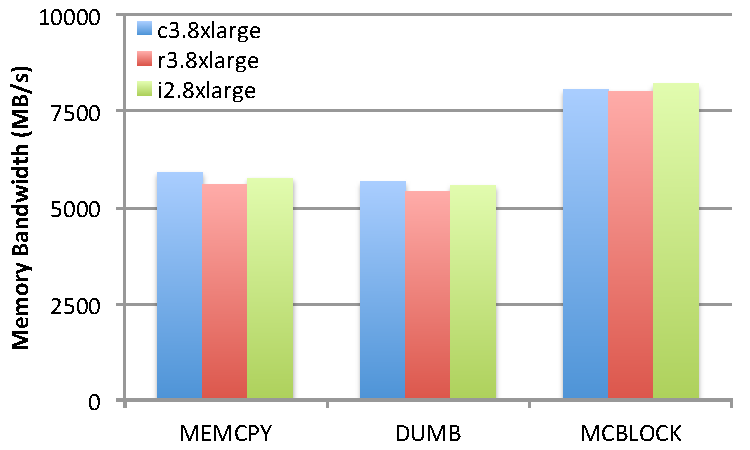
\includegraphics[width=6cm]{benchmark_mem}} 
  \hspace{5pt}
 \subfloat[Disk IO Benchmark]{ 
    \label{fig:subfig:benchmark_disk}  
    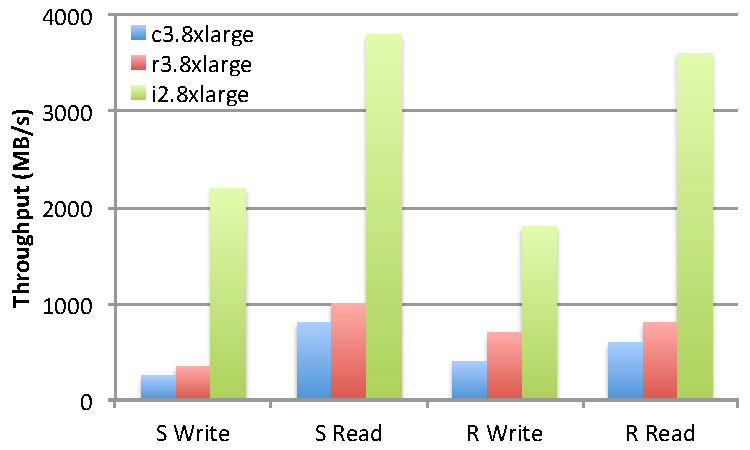
\includegraphics[width=6cm]{benchmark_disk}} 
  \caption{Benchmark of CPU, memory and disk IO for c3.8xlarge, r3.8xlarge and i2.8xlarge instances.} 
  \label{fig:instance_benchmark} 
\end{figure*}


Many people perceive computing resources on AWS as of equal performance across instance types. For example, one vCPU on c3.8xlarge instances is expected to have the same performance as one vCPU on r3.8xlarge instances; the SSD storage on c3.8xlarge instances is expected to have the same performance as the SSD storage on r3.8xlarge instances. We use UnixBench \footnote{The source code is available from \url{http://code.google.com/p/byte-unixbench/}.}, MBW \footnote{The man page is available from \url{http://manpages.ubuntu.com/manpages/karmic/man1/mbw.1.html}.}, and IOZone \footnote{The source code is available from \url{http://www.iozone.org}.} to benchmark the CPU, memory and disk IO performance of the three instance types being used in this study. 

UnixBench is a benchmark suite that can be used to evaluate the overall performance of Unix-like systems. The original version of UnixBench was developed in 1983 at Monash University. Afterwards it was updated and revised by many people over the years. In this study we used the version ``byte-unixbench'' available from the Google Code website. In the UnixBench benchmark suite, several different tests are carried out to evaluate the performance of the system. Based on the scores of the above-mentioned different tests, a system level score (System Benchmarks Index Score) is calculated. In this study, we use this system level score to compare the CPU performance of different VM instances. The test results are presented in Figure \ref{fig:subfig:benchmark_cpu}. In the 1-thread test, all three instance types achieve similar scores. In the 32-thread test, the c3.8xlarge instance achieves the best score, followed by r3.8xlarge and then i2.8xlarge. 

MBW measures available memory bandwidth by copying large arrays of data in memory. In the MEMCPY test, we measure the speed achieved while copying a 128 MB array from one area of memory to another. In the DUMB test, we allocate two arrays of 128 MB, then copy the value of each element in the first array to the corresponding element in the second array with operations such as "b[i] = a[i]". The MCBLOCK test is similar to the MEMCPY test, but the copy operation is carried out in 4096-byte blocks. As shown in Figure \ref{fig:subfig:benchmark_mem}, all three instance types have similar memory performance in all three tests. The r3.8xlarge instance performs slightly worse in all three tests, but the performance difference is insignificant. 

IOZone benchmarks the performance of the underlying file system by generating and measuring a variety of file operations. Different scientific computing applications have different disk IO patterns. In general, applications dealing with large input / output files (such as large scale sorting) demands sequential IO capability, while applications dealing with a large number of small input / output files (such as Montage) demands random IO capability. In the sequential IO test, we use two 256 GB test files as the input to make sure that they will not fit into the memory of the instance being tested. In the random IO test, we use 2,000,000 small files ranging from 4 KB to 40 MB as the input, and the total size of the input files is 512 GB. As shown in Figure \ref{fig:subfig:benchmark_disk}, the disk IO performance is dramatically different for the three instance types. In the sequential write (S Write) test, the sequential write throughput of the RAID0 device on c3.8xlarge instances is only 1/2 of the sequential write throughput of the RAID0 device on r3.8xlarge instances. Since both c3.8xlarge and r3.8xlarge instance types have 2 x 320 GB SSD storage, it is obvious that the SSD disks being used for c3.8xlarge instances are different from the SSD being used for r3.8xlarge instances. The sequential write throughput of the RAID0 device on i2.8xlarge instances is 4 times the sequential write throughput of the RAID0 device on r3.8xlarge instances. Since the i2.8xlarge instance has 8 SSD disks while the r3.8xlarge has 2 SSD disks, it is quite possible that the SSD disks being used for r3.8xlarge and i2.8xlarge instances are the same. Similar trends are also observed in the tests for sequential read (S Rread), random write (R Write), and random read (R Read).


\section{Performance Evaluation of DEWE v2}
\label{v2_sec:dewe_v2_performance}


\subsection{Scheduling vs Pulling}
\label{sec:subsec:scheduling_vs_pulling}


\begin{figure*}[t!]
\centering
\vspace{-10pt}
 \subfloat[Concurrent Threads]{ 
    \label{fig:subfig:dewe2_threads}  
    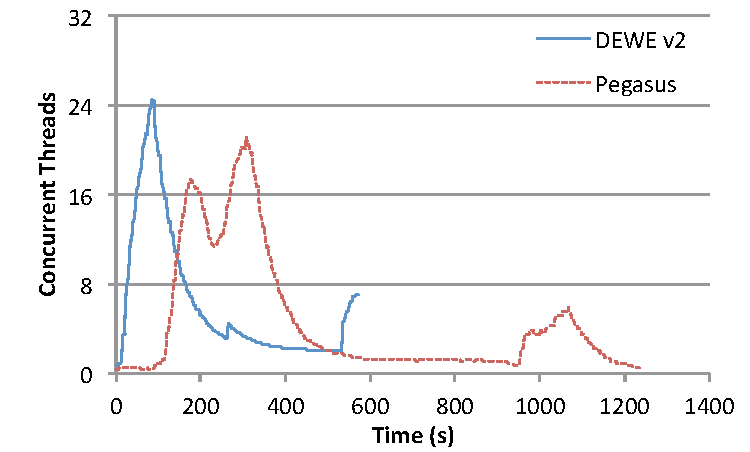
\includegraphics[width=6cm]{compare_threads}} 
 \hspace{5pt}
 \subfloat[CPU Utilization]{ 
    \label{fig:subfig:dewe_v2_cpu}  
    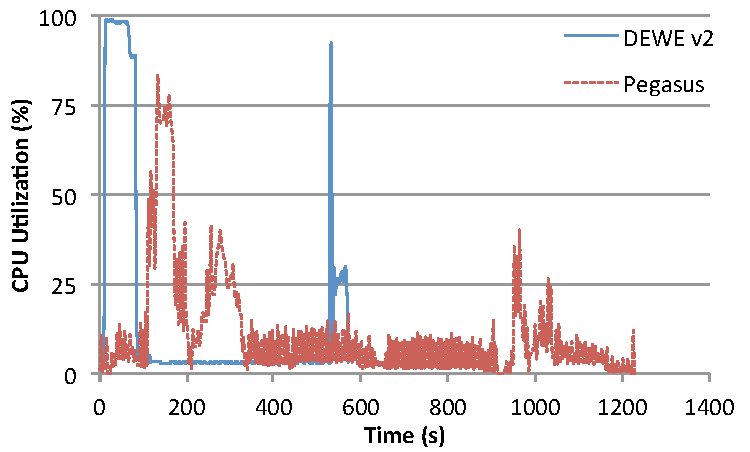
\includegraphics[width=6cm]{compare_cpu}}
 \hspace{5pt}
 \subfloat[Disk Write Operations]{ 
    \label{fig:subfig:dewe_v2_disk_writes}  
    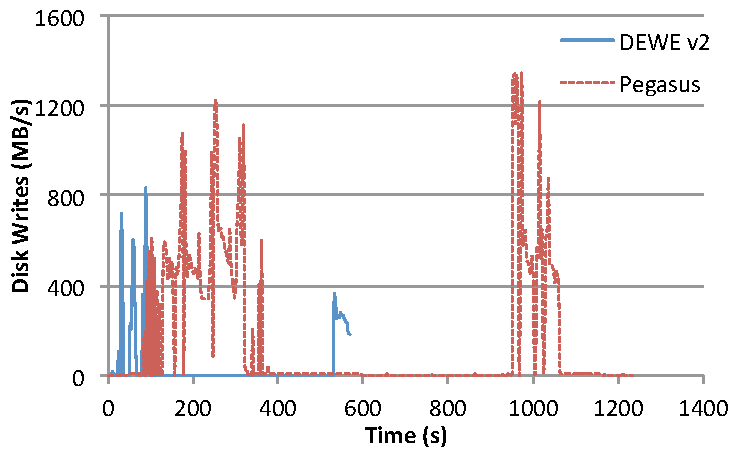
\includegraphics[width=6cm]{compare_disk_writes}} 
  \caption{Resource consumption patterns of one 6.0 degree Montage workflow running on a single-node cluster with DEWE v2 and Pegasus. The instance type being used is c3.8xlarge.} 
  \label{fig:compare_graphs} 
\end{figure*}



\begin{figure*}[t!]
\centering
\vspace{-10pt}
 \subfloat[Total Execution Time]{ 
    \label{fig:subfig:multi_run_makespan}  
    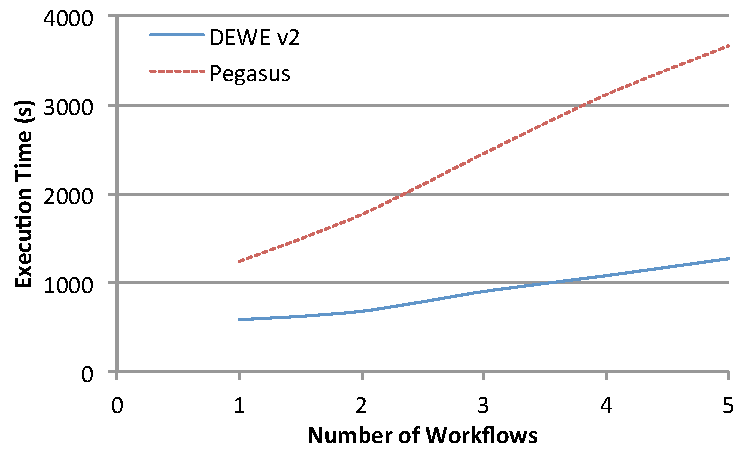
\includegraphics[width=6cm]{multi_run_makespan}} 
 \hspace{5pt}
 \subfloat[Total CPU Time]{ 
    \label{fig:subfig:multi_run_cpu_time}  
    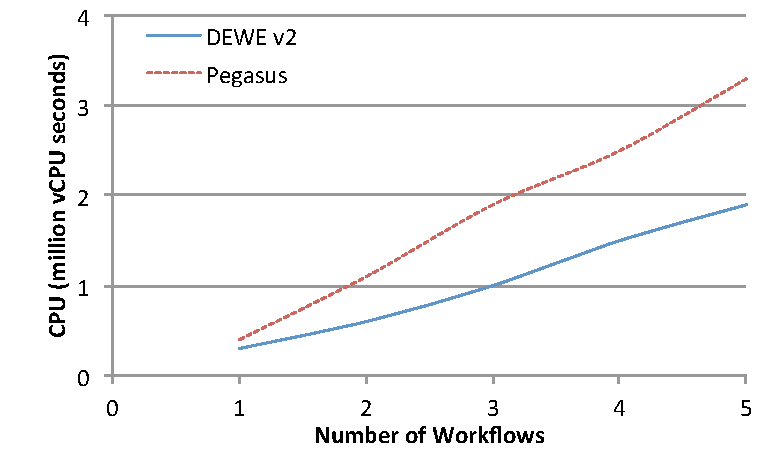
\includegraphics[width=6cm]{multi_run_cpu_time}} 
  \hspace{5pt}
 \subfloat[Total Disk Writes]{ 
    \label{fig:subfig:multi_run_disk_writes}  
    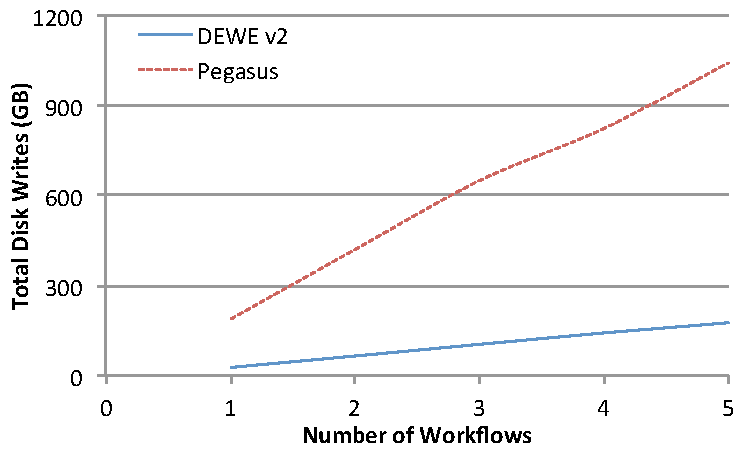
\includegraphics[width=6cm]{multi_run_disk_writes}} 
  \caption{Resource consumption of multiple 6.0 degree Montage Workflow running on a single-node cluster with Pegasus and DEWE v2. The instance type being used is c3.8xlarge.} 
  \vspace{-15pt}
  \label{fig:multi_run} 
\end{figure*}

In this paper, we use Pegasus as a representative of the scheduling-based workflow execution engines. 

Figure \ref{fig:compare_graphs} shows the resource consumption patterns of one 6.0 degree Montage workflow running on a single-node cluster with DEWE v2 and Pegasus. The experiments are carried out on AWS EC2 in its us-east-1 region. The instance type being used is c3.8xlarge. The storage being used is the instance-store SSD volumes with RAID 0 configuration. To eliminate the impact of network latency, the required input files are downloaded to the storage device before the experiments. Although the c3.8xlarge instance has 32 vCPU, the maximum number of concurrent threads observed is 25 for DEWE v2 and 20 for Pegasus. The maximum CPU utilization observed is 100\% for DEWE v2 and 80\% for Pegasus. This indicates that DEWE v2 is more efficient in utilizing CPU resources. The observed disk write operations for Pegasus is much higher than DEWE v2, indicating that Pegasus carries out more disk I/O activities than DEWE v2. For DEWE v2, the average makespan is 600 seconds. For Pegasus, the average make span is 1240 seconds, which is significantly longer. 

Figure \ref{fig:multi_run} shows the resource consumption of multiple 6.0 degree Montage workflows running on a single node cluster with Pegasus and DEWE v2. The instance being used  is c3.8xlarge on AWS EC2 in the us-east-1 region. The desired number of workflows are submitted to the workflow management system in one batch. The required input files are downloaded to the storage devices on the instance before the experiments. Total execution time (Figure \ref{fig:subfig:multi_run_makespan}) refers to the time needed to finish the execution of the workflows, regardless of the actual resource utilization rate on the worker nodes. When the number of workflows increases, the total execution time increases linearly. Total CPU time (Figure \ref{fig:subfig:multi_run_cpu_time}) refers to the actual CPU time spent on job execution activities, which is calculated by integrating the actual CPU utilization rate over the entire workflow execution period on all CPUs. Total disk writes (Figure \ref{fig:subfig:multi_run_disk_writes}) refers to the amount of data being written to the file system, which is calculated by integrating the actual disk write throughput over the entire workflow execution period. when the number of workflows increases, both total CPU time and total disk writes increase linearly. In general, Pegasus consumes a lot more computing resource (such as CPU time and disk writes) than DEWE v2, resulting in much longer execution time. For example, the execution time of five 6.0 degree Montage workflows being run with DEWE v2 is approximately the same as the execution time of one 6.0 degree Montage workflow being run with Pegasus. In other words, DEWE v2 can achieve 80\% speed-up when running multiple scientific workflows in parallel with the same cluster configuration. 



\subsection{Workflow Submission Intervals}
\label{sec:subsec:submission}


\begin{figure}[!t]
	\centering
	\hspace{-10pt}
	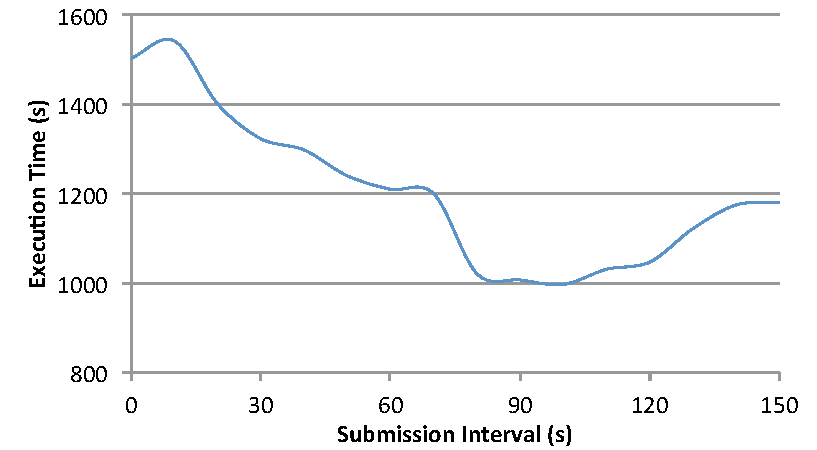
\includegraphics[width=8.5cm]{dewe_v2_submission_intervals}
    \vspace{5pt}
	\caption{Execution time of five 6.0 degree Montage Workflow running on a single-node cluster with DEWE v2. The instance type being used is c3.8xlarge.}
	\label{fig:dewe_v2_submission}
\end{figure}




A 6.0 degree Montage workflow demands different computing resources in different stages. When executing a large scale workflow ensemble with many workflows on the same cluster, it is possible to optimize resource utilization by controlling the workflow submission intervals so that different workflows in the workflow ensemble do not demand the same computing resource at the same time. In this test, we run a workflow ensemble with five 6.0 degree Montage workflows with DEWE v2 on a single-node cluster with both the master daemon and worker daemon on the same node. The test includes submitting all five workflows in one batch (batch submission), or submitting the five workflows one after another at fixed intervals (incremental submission). Batch submission can be considered as a special case of incremental submission where the submission interval is zero. As shown in Figure \ref{fig:dewe_v2_submission}, the time needed to execute all five workflows decreases when the submission interval increases, then increases again when the submission interval is greater than 100 seconds. In this particular test case, 34\% speed up can be achieved by setting the submission interval to 100 seconds.

Figure \ref{fig:dewe_v2_submission_pattern} shows the resource consumption patterns of the test workflow ensemble with five 6.0 degree Montage workflows running on a single node cluster with DEWE v2. Due to space limits we only show results with workflow submission intervals of 0, 50 and 100 seconds. As shown in Figure  \ref{fig:subfig:dewe_v2_submission_cpu}, when we increase the workflow submission interval, we change the CPU utilization pattern in the system. When submission interval is 0 second, the CPU utilization exhibits a clear three-stage pattern, with significant resource under-utilization in the second stage. This is very similar to the CPU utilization pattern in a single workflow. When submission interval is 100 seconds, such three-stage pattern is no longer obvious. This is because different types of jobs from different workflows can be executed in parallel, resulting in an increase in average CPU utilization across the whole execution time. The same result is also observed in disk I/O activities, which is reflected in both disk writes (Figure \ref{fig:subfig:dewe_v2_submission_disk_writes}) and disk reads (Figure \ref{fig:subfig:dewe_v2_submission_disk_reads}). Due to the increase in resource utilization, shorter execution time can be achieved with well-designed incremental submission techniques. 

\subsection{System Robustness}
\label{sec:subsec:rubustness}

We carry out two tests to examine the robustness of DEWE v2. In one test, we run one 6.0 degree Montage workflow with DEWE v2 on a single-node cluster with both the master daemon and worker daemon on the same node. During the execution of the workflow, we introduce interruptions to the system by killing the worker daemon and then starting it again 5 seconds later. In the other test, we run one 6.0 degree Montage workflow with DEWE v2 on a two-node cluster with NFS as the shared file system. One of the nodes has both the master daemon and the worker daemon, while the other node has only the worker daemon. However, at any time there is only one worker daemon running. During the execution of the workflow, we introduce interruptions to the system by killing the worker daemon on one node, then starting the worker daemon on the other node 5 seconds later. 

In both tests, interrupted jobs are automatically resubmitted for execution after timeouts. DEWE v2 is capable of completing the execution of the workflow, regardless of number of interruptions. When the interruptions are introduced during the execution of none-blocking jobs such as mProjectPP and mDiffFit, the increase in makespan roughly equals to the total duration of the interruptions. This is because DEWE v2 can resume execution of the workflow as soon as the worker daemon restarts, without the need to wait for the timeout of the interrupted jobs. When the interruptions are introduced during the execution of blocking jobs such as mConcatFit and mBgModel, the increase in makespan roughly equals to the sum of the timeout settings of the interrupted jobs. This is because DEWE v2 must wait for the timeout of the interrupted jobs to resume execution of the workflow.

DEWE v2's capability of resuming workflow execution after interruption of the worker daemon opens the door for dynamic resource provisioning. During the execution of large scale workflow ensembles, researchers can dynamically adjust the number of worker nodes in a cluster to meet both deadline and cost constrains. When there are a large number of none-blocking jobs in the queue, more worker nodes can be added to the cluster to speed up the execution. When there are a limited number of blocking jobs in the queue, some worker nodes can be removed from the cluster to reduce cost. Such dynamic resource provisioning strategy might not be effective for public clouds with a charge-by-hour model (such as AWS), but can be useful for public clouds with a charge-by-minute model (such as Google Compute Engine). In this paper, we carry out all our experiments on AWS, therefore we are not able to explore further on this topic.



\section{Resource Provisioning Strategy}
\label{sec:provision}

\begin{figure*}[t!]
\centering
\vspace{-10pt}
 \subfloat[CPU Utilization]{ 
    \label{fig:subfig:dewe_v2_submission_cpu}  
    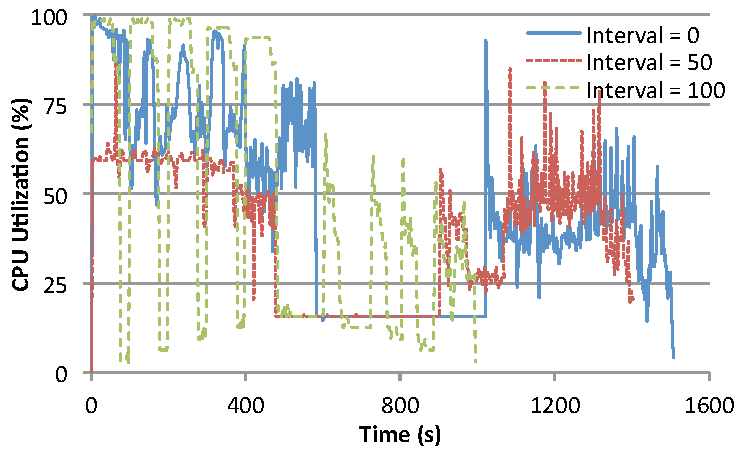
\includegraphics[width=6cm]{dewe_v2_submission_cpu}} 
  \hspace{5pt}
 \subfloat[Disk Write Operations]{ 
    \label{fig:subfig:dewe_v2_submission_disk_writes}  
    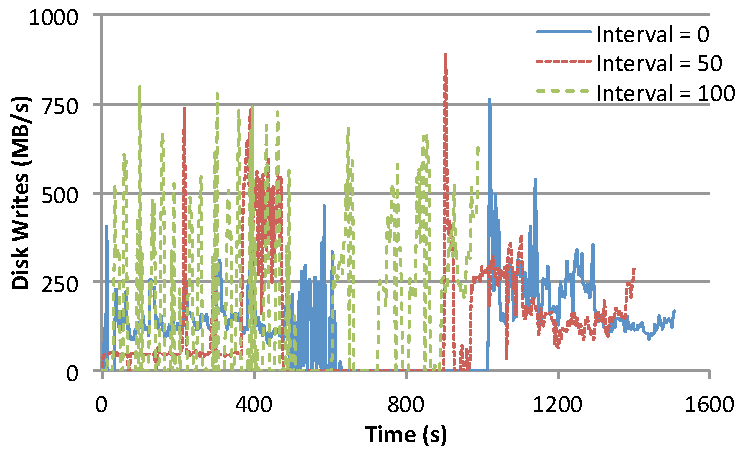
\includegraphics[width=6cm]{dewe_v2_submission_disk_writes}} 
  \hspace{5pt}
 \subfloat[Disk Read Operations]{ 
    \label{fig:subfig:dewe_v2_submission_disk_reads}  
    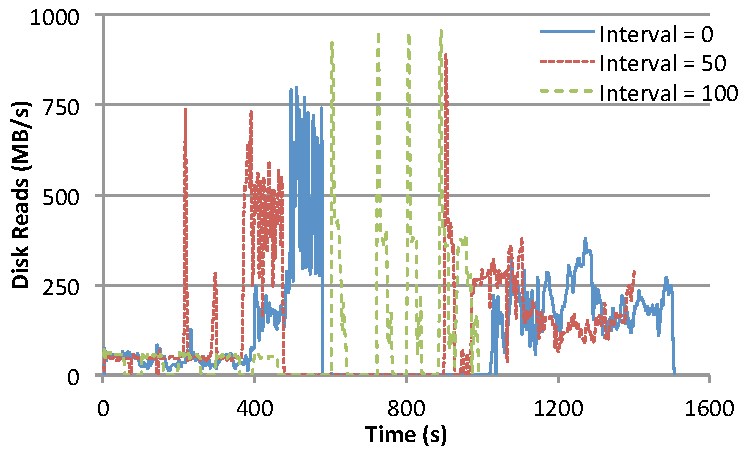
\includegraphics[width=6cm]{dewe_v2_submission_disk_reads}} 
  \caption{Resource consumption patterns of five 6.0 degree Montage workflows running on a single node cluster with DEWE v2. The workflow submission intervals are 0, 50 and 100 seconds.} 
  \label{fig:dewe_v2_submission_pattern} 
\end{figure*}

\begin{figure*}[t!]
\centering
\vspace{-10pt}
 \subfloat[CPU Utilization]{ 
    \label{fig:subfig:10_runs_cpu}  
    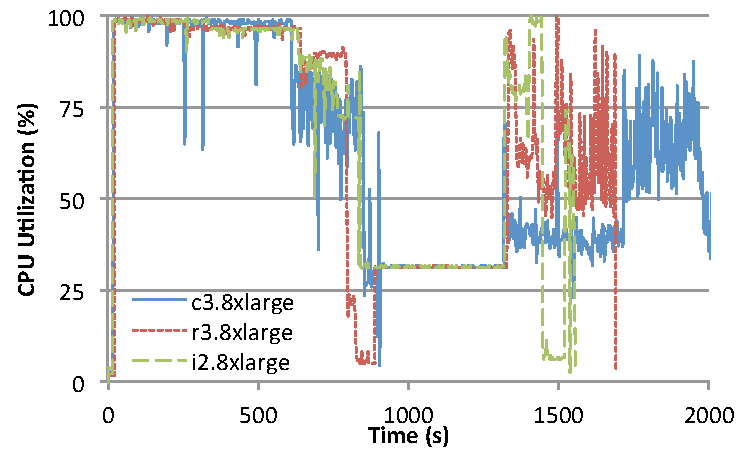
\includegraphics[width=6cm]{10_runs_cpu}} 
  \hspace{5pt}
 \subfloat[Disk Write Operations]{ 
    \label{fig:subfig:10_runs_disk_writes}  
    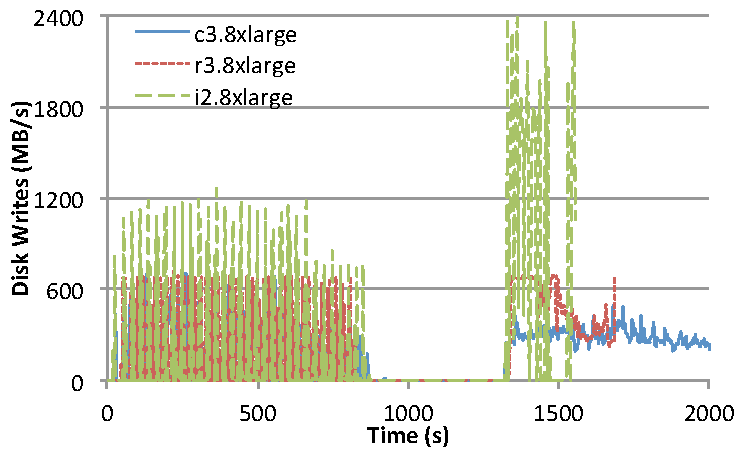
\includegraphics[width=6cm]{10_runs_disk_writes}} 
    \hspace{5pt}
 \subfloat[Disk Read Operations]{ 
    \label{fig:subfig:10_runs_disk_reads}  
    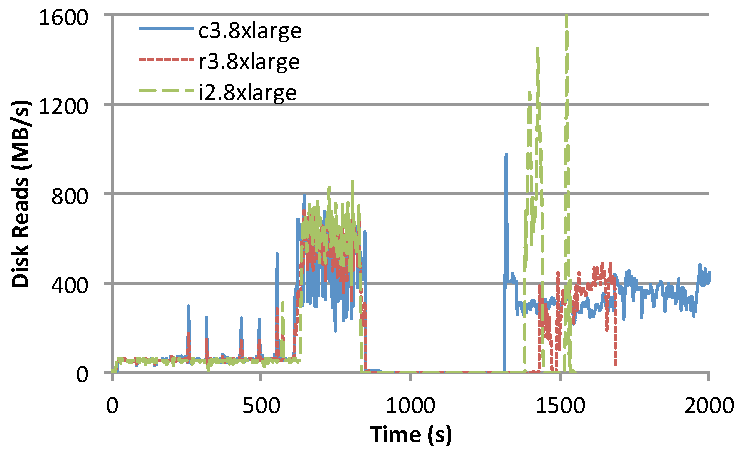
\includegraphics[width=6cm]{10_runs_disk_reads}} 
  \caption{Resource consumption patterns of ten 6.0 degree Montage workflows running on a single node cluster with DEWE v2. The instance type being used are c3.8xlarge, r3.8xlarge and i2.8xlarge.} 
  \label{fig:10_runs} 
\end{figure*}

In this section, we propose a two-step strategy to provision computing resources for large scale scientific workflow ensembles with both cost and deadline constraints. We begin with small scale experiments to profile the resource consumption patterns of the workflow ensemble when the underlying computing nodes are fully utilized. Based on the small scale testing results we derive the performance index of a worker node. Then we use the performance index to determine the number of worker nodes needed for the actual large scale experiments. To simplify our discussions, all the tests presented in this section are carried out with batch submission rather than incremental submission.

\subsection{Profiling}
\label{sec:subsec:pattern}

 
 \begin{figure*}[t!]
\centering
\vspace{-10pt}
 \subfloat[CPU Utilization]{ 
    \label{fig:subfig:2_node_cpu}  
    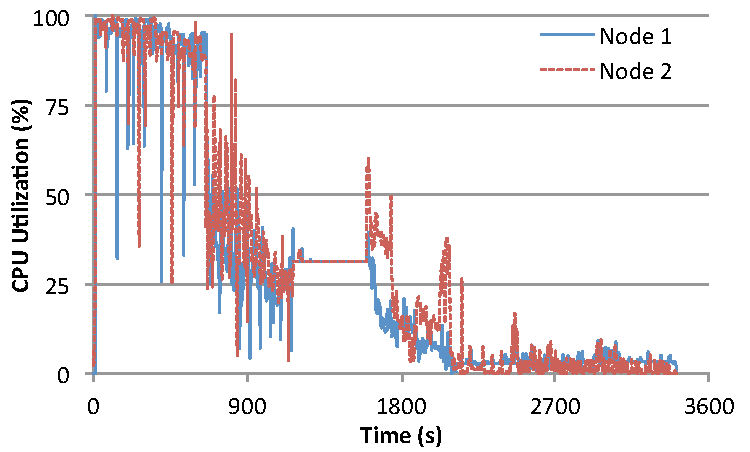
\includegraphics[width=6cm]{2_node_cpu}} 
  \hspace{5pt}
 \subfloat[Disk Write Operations]{ 
    \label{fig:subfig:2_node_disk_writes}  
    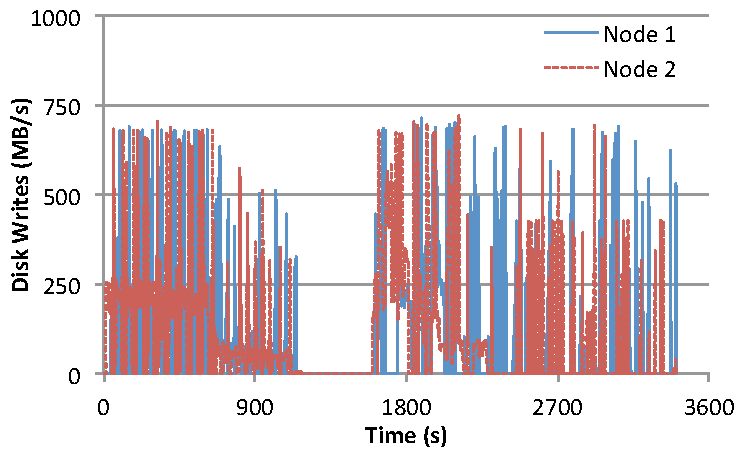
\includegraphics[width=6cm]{2_node_disk_writes}} 
  \hspace{5pt}
 \subfloat[Disk Read Operations]{ 
    \label{fig:subfig:2_node_disk_reads}  
    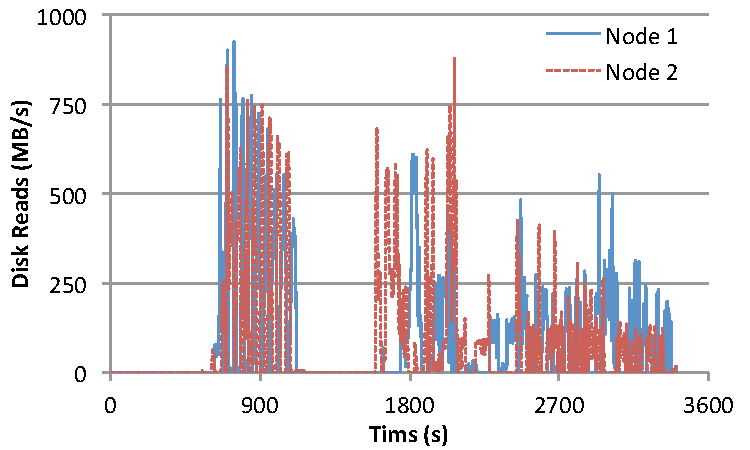
\includegraphics[width=6cm]{2_node_disk_reads}} 
\caption{Resource consumption patterns of 20 6.0 degree Montage workflows running on a 2-node cluster with DEWE v2. The instance type being used is r3.8xlarge. The shared file system is NFS.}   
  \label{fig:2_node_pattern} 
\end{figure*}

To come up with a resource provisioning strategy for executing large scale scientific workflow ensembles in public clouds, we use both single-node tests and multi-node tests to profile the resource consumption pattern of multiple workflows running in parallel. 


We use the c3.8xlarge, r3.8xlarge, and i2.8xlarge instances on AWS EC2 for our experiments. Table \ref{tbl:instance_type} lists the specifications of the selected instance types. On all of the selected instance types, the storage devices are SSD-backed instance store volumes (storage from disks that are physically attached to the host computer). To achieve the best disk I/O performance, we combine all the instance store volumes available on the instance in a RAID 0 configuration. All the workflow related disk I/O operations are configured to occur on the RAID 0 device. The file system being used on all worker nodes is ext4. Benchmark testings reveal that all three instance types have similar CPU and memory performance. However, there exists significant difference in the disk I/O performance of the RAID 0 device, which is shown in Table \ref{tbl:instance_disk_io}. 


In the single-node tests, we run up to ten 6.0 degree Montage workflows on a single-node cluster with DEWE v2. The largest workload contains 85,860 jobs, 14,440 input files with a total size of 40 GB, and 228,500 intermediate files with a total size of 350 GB. 

Figure \ref{fig:10_runs} shows the resource consumption pattern of ten 6.0 degree Montage workflows running on a single-node cluster with DEWE v2. During the first stage, the workflow is CPU intensive, as evidenced by the 100\% CPU utilization rate on all three instance types (Figure \ref{fig:subfig:10_runs_cpu}). If we look at the disk write operations alone (Figure \ref{fig:subfig:10_runs_disk_writes}), we would think that the workflow is I/O intensive during this stage. However, this stage takes approximately the same amount of time on all three instance types, regardless of the significant difference in their write throughput. This indicates that CPU is the real bottleneck during this stage. The operating system caches the disk writes and flushes them to the disk in batches, resulting in the intermittent disk writes at full capacity. During the second stage, the workflow is neither CPU intensive nor I/O intensive, as evidenced by the low CPU utilization rate and zero disk writes. The progress of the workflow is controlled by the single-thread mConcatFit and mBgModel jobs. During the third stage, the workflow is  I/O intensive. The i2.8xlarge instance, with the highest I/O capacity, finishes executing this stage first, following by the r3.8xlarge and the c3.8xlarge instances, according to their I/O capacities.




\begin{figure*}[t!]
\centering
\vspace{-10pt}
 \subfloat[Single-Node Cluster]{ 
    \label{fig:subfig:single_node_multi_runs}  
    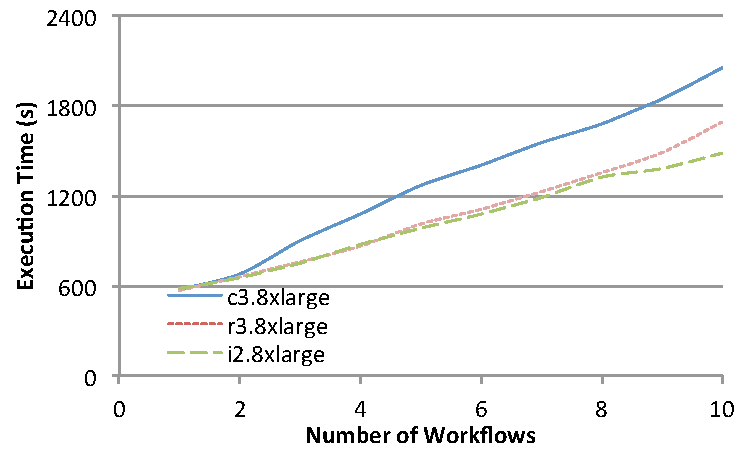
\includegraphics[width=6cm]{single_node_multi_runs}} 
  \hspace{5pt}
 \subfloat[Multi-Node Cluster]{ 
    \label{fig:subfig:multi_node_20_runs}  
    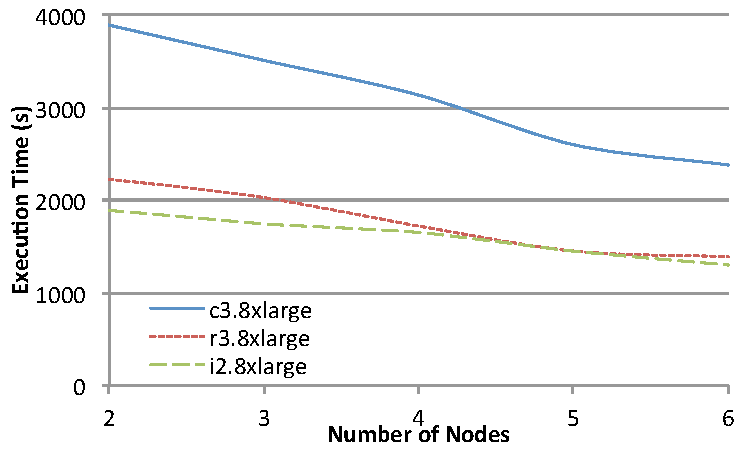
\includegraphics[width=6cm]{multi_node_20_runs}} 
  \hspace{5pt}
 \subfloat[Performance Degradation]{ 
    \label{fig:subfig:performance_degradation}  
    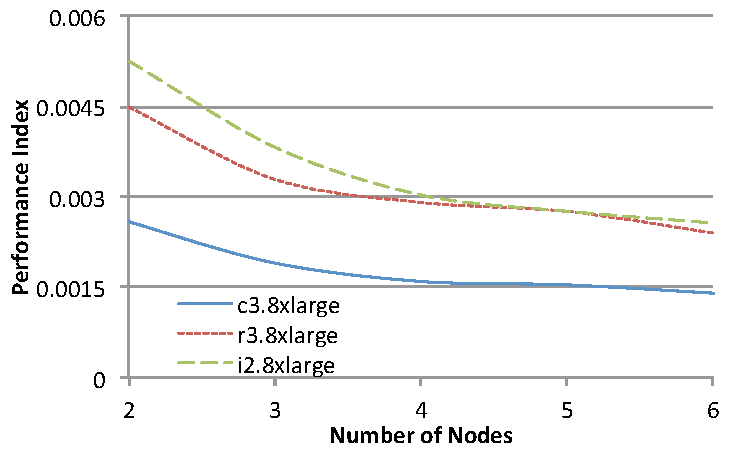
\includegraphics[width=6cm]{performance_index}} 
\caption{The impact of workload and cluster size on the performance of the cluster. On the single-node clusters, we run up to 10 6.0 degree Montage workflows. On the multi-node clusters, we run 20 6.0 degree Montage workflows in one batch.}   
  \label{fig:small_scale_summary} 
\end{figure*}

In the multi-node tests, we run twenty 6.0 degree Montage workflows on multi-node clusters with DEWE v2. The workload contains 172,720 jobs, 28,880 input files with a total size of 80 GB, and 457,000 intermediate files with a total size of 700 GB. In a multi-node cluster, one of the nodes runs both the master daemon and the worker daemon, while the other nodes run the worker daemon. All nodes share its storage with the other nodes using NFS. For example, in a two-node cluster, node A has a locally-mounted folder A and a NFS-mounted folder B, while node B has a NFS-mounted folder A and a locally mounted folder B. In order to balance the pressure on disk I/O, we evenly distribute the input files onto different nodes. For example, in a 2-node cluster, the input files for 10 workflows are located on node A while the input files for the other 10 workflows are located on node B.

Figure \ref{fig:2_node_pattern} shows the resource consumption pattern in a 2-node r3.8xlarge cluster. Similar to the resource utilization pattern in a single-node cluster, the first stage is controlled by the CPU resource and the second stage is controlled by the single-thread mConcatFit and mBgModel jobs. During the third stage, the CPU utilization on both nodes is extremely low, the progress of the workload is controlled by the large number of intermittent disk I/O operations. The peak of these I/O operations is 750 MB/s for both read and write operations, indicating the performance of NFS is the bottleneck of the cluster.  


\subsection{Determining Cluster Size}
\label{sec:subsec:Performance index}

Figure \ref{fig:small_scale_summary} shows the impact of workload and cluster size on the performance of the cluster. On the single-node cluster, the size of the cluster remains the same. As the number of workflows increases, the execution time increases linearly (Figure \ref{fig:subfig:single_node_multi_runs}). On the multi-node cluster, the size of the workload remains the same. As the number of worker nodes increases, the execution time decreases linearly (Figure \ref{fig:subfig:multi_node_20_runs}). 

The performance index of the worker nodes in a multi-node cluster can be defined as the execution speed of the workflow on a single node, that is

\begin{equation}
P =\frac{W}{N * T}
\label{eq:performance_index} 
\end{equation}
\\
where P is the performance index (workflow per second per node), W is the number of workflows running on the cluster, N is the number of worker nodes in the cluster, and T is the execution time needed for N workflows. A simple way to read this is how much of a workflow can be completed by one worker node in one second. As shown in Figure \ref{fig:subfig:performance_degradation}, as the number of worker nodes increases, the performance index decreases. The phenomenon is commonly observed in clusters, and is referred to as clustering performance degradation. In our test case, the observed clustering performance degradation gradually converges when the number of worker nodes is greater than 4. Based on Figure \ref{fig:subfig:performance_degradation}, we estimate that the performance indexes for large scale clusters are 0.0015, 0.0024, and 0.0026 for clusters with c3.8xlarge, r3.8xlarge, and i2.8xlarge instance types.

Based on Equation \ref{eq:performance_index}, we can estimate the number of worker nodes needed to execute a large scale scientific workflow ensemble with deadline constraints using the following formula:

\begin{equation}
N =\frac{W}{P * T}
\label{eq:node_estimation} 
\end{equation}
\\
where N is the desired number of worker nodes in the cluster, W is the number of workflows in the workflow ensemble, P is the performance index of the EC2 instance type, and T is the desired execution time. 



\subsection{Large Scale Experiments}
\label{v2_sec:subsec:large_scale}


\begin{table}[t!]
\caption{Cluster Configurations}
\label{tbl:cluster_config}
\centering
\begin{tabular}{|p{1.4cm}|p{0.9cm}|p{0.9cm}|p{0.9cm}|p{0.9cm}|p{0.9cm}|}
\hline
Cluster & Nodes & vCPU & Memory (TB) & Storage (TB)&Price (USD/hr)\\ \hline
c3.8xlarge & 40 & 1280 & 2.40 & 25.6 & 67.2\\ \hline
r3.8xlarge & 25 & 800  & 6.10 & 16.0 & 70.0\\ \hline
i2.8xlarge & 23 & 768  & 5.61 & 147.2 & 156.7\\ \hline
i2.8xlarge B & 10 & 320  & 2.44 & 64.0 & 68.2\\ \hline
\end{tabular}
\end{table}

\begin{figure*}[t!]
\centering
\vspace{-10pt}
 \subfloat[CPU Utilization]{ 
    \label{fig:subfig:large_scale_cpu}  
    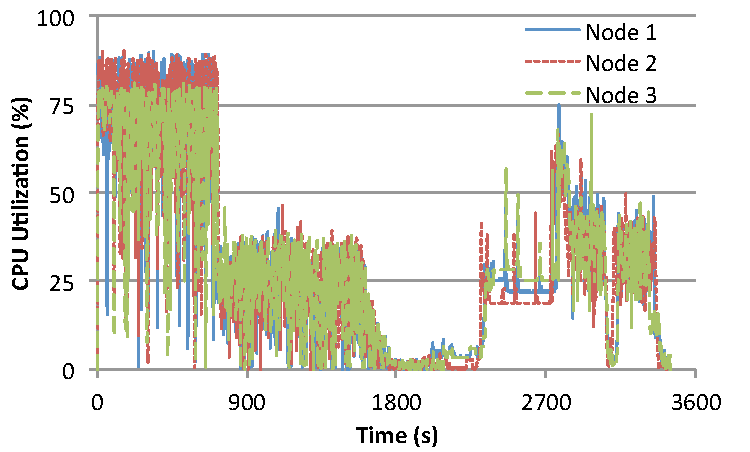
\includegraphics[width=6cm]{large_scale_cpu}} 
  \hspace{5pt}
 \subfloat[Disk Write Operations]{ 
    \label{fig:subfig:large_scale_disk_writes}  
    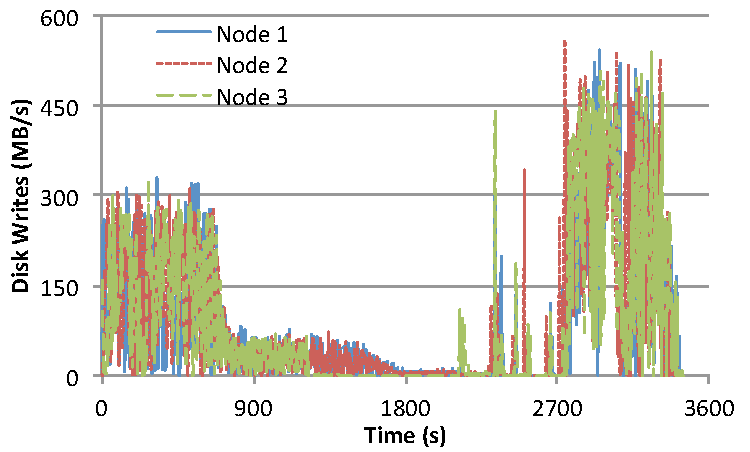
\includegraphics[width=6cm]{large_scale_disk_writes}} 
  \hspace{5pt}

 \subfloat[Disk Read Operations]{ 
    \label{fig:subfig:large_scale_disk_reads}  
    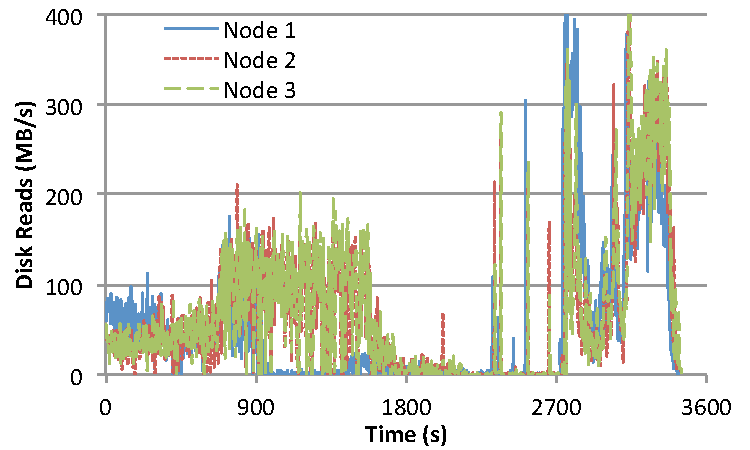
\includegraphics[width=6cm]{large_scale_disk_reads}} 
  \caption{Resource consumption patterns of 200 6.0 degree Montage workflows running on a 25-node cluster with DEWE v2. The instance type being used is r3.8xlarge.} 
  \label{fig:large_scale_pattern} 
\end{figure*}


\begin{figure*}[t!]
\centering
\vspace{-10pt}
 \subfloat[Execution Time]{ 
    \label{fig:subfig:large_scale_runs}  
    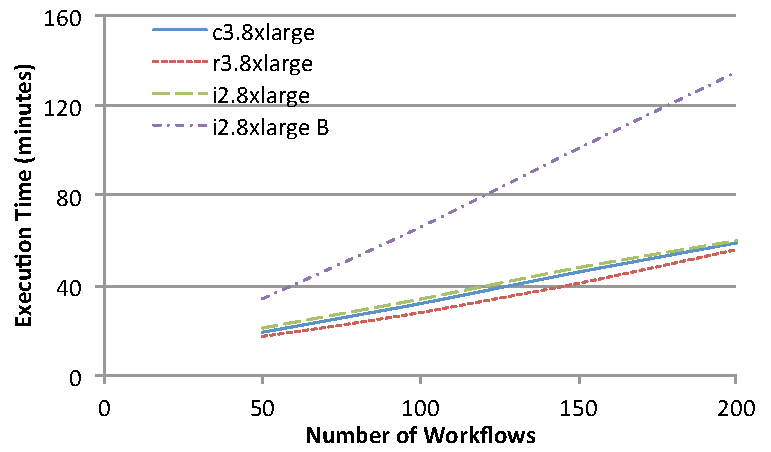
\includegraphics[width=6cm]{large_scale_runs}} 
  \hspace{5pt}
 \subfloat[Performance Index]{ 
    \label{fig:subfig:large_scale_performance}  
    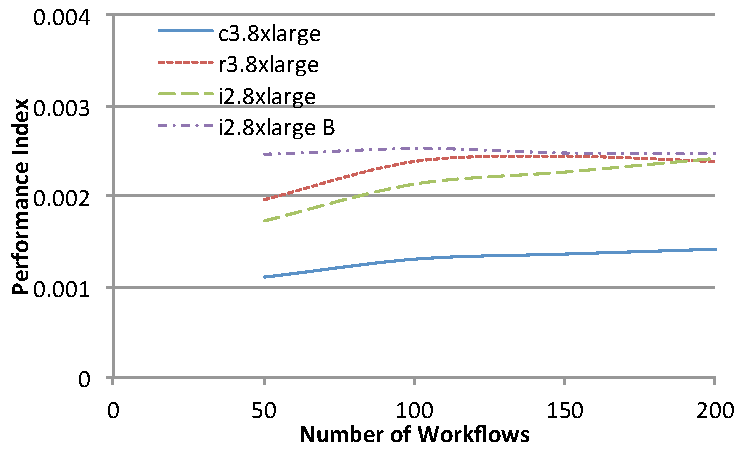
\includegraphics[width=6cm]{large_scale_performance_index}} 
  \hspace{5pt}
 \subfloat[Price per Workflow]{ 
    \label{fig:subfig:large_scale_price}  
    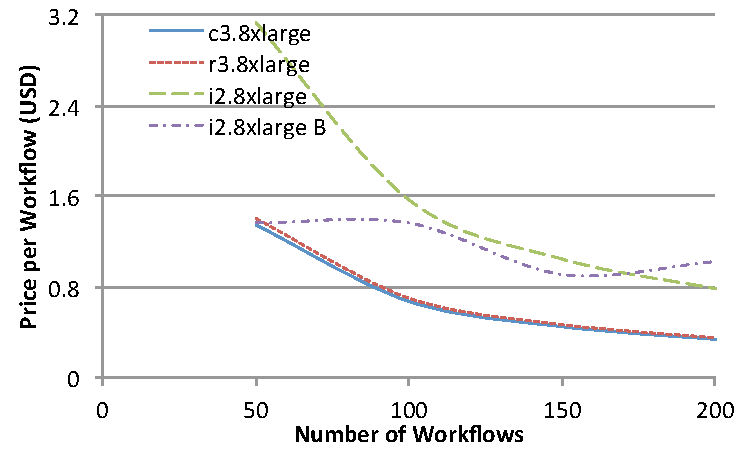
\includegraphics[width=6cm]{large_scale_price}} 
\caption{Summary of the large scale experiments.}   
  \label{fig:large_scale_runs} 
\end{figure*}

We use large scale experiments to evaluate the above-mentioned resource provisioning strategy. The largest workflow ensemble includes 200 6.0 degree Montage workflows, which contains 1,717,200 jobs, 288,800 input files, and 4,570,000 intermediate files. Approximately 7.0 TB data is written to the underlying storage during the execution. 

In order to meet both cost and deadline constraints, we design our clusters with the goal to complete the largest workload ensemble (W = 200) within an hour. This is because users pay for EC2 instances by the hour, and any partial hour usage will be charged as a full hour. The time constrain T is set to 3300 seconds (55 minutes) because we would like to have some flexibility in the execution time. Based on Equation \ref{eq:node_estimation}, the estimated number of worker nodes are 40, 25, and 23 for c3.8xlarge, r3.8xlarge and i2.8xlarge instance types. An additional cluster i2.8xlarge B with the i2.8xlarge instance type and 10 nodes is also tested as a comparison. We use 10 nodes for the i2.8xlarge B cluster because it has approximately the same hourly price as the c3.8xlarge and r3.8xlarge clusters. Table \ref{tbl:cluster_config} lists the four test clusters along with their total amount of vCPU, memory and storage, as well as the hourly price as calculated with the on-demand instance prices. 

In our previous experiments, we use NFS as the share file system between worker nodes. This requires each and every worker node to share its local storage via NFS, and mount the NFS shares from other nodes, resulting in an N-to-N mapping between worker nodes. As the size of the cluster grows, the configuration of the cluster becomes increasingly complex, resulting in unbalanced utilization. In the large scale experiments, we use MooseFS \cite{moosefs} as the shared file system between worker nodes. All the worker nodes are configured to be a MooseFS trunk server. Using cloud-init scripts, the worker nodes automatically join the storage pool and mount the MooseFS file system when the instances are being launched. Furthermore, the required input files are copied to the shared file system before the experiments. Therefore, the test results only include the execution time of the workflow ensemble. As a distributed file system, MooseFS has the option to store one file with multiple copies on different storage devices. In order to save storage space, each file has only one copy in our experiments. The worker nodes mount the shared file system as a POSIX-compliant file system. When executing a particular job, the worker daemon has no knowledge about the actual location of the input and output files. In order words, data locality can not be assumed in our experiments. However, it is safe to assume that statistically all worker nodes have equal access to the underlying shared file system. 


Figure \ref{fig:large_scale_pattern} shows the resource consumption pattern of 200 6.0 degree Montage workflows running on the r3.8xlarge cluster. The cluster includes 25 worker nodes, but we only present data from three worker nodes. As shown in the figure, all three worker nodes have the same the resource consumption patterns, which is similar to the resource consumption pattern on a single-node cluster (Figure \ref{fig:10_runs}). This is also true for other worker nodes not shown in the figure. This indicates that the workload is evenly distributed across the cluster. The cluster behaves in a way that is similar to a supercomputer. 


Figure \ref{fig:large_scale_runs} shows the execution time, performance index, and price per workflow for workflow ensembles with different number of 6.0 degree Montage workflows. For all clusters, the execution time increases linearly as the number of workflows in the workflow ensemble increases (Figure \ref{fig:subfig:large_scale_runs}). On clusters c3.8xlarge, r3.8xlarge and i2.8xlarge, the workflow ensemble with 200 6.0 degree Montage workflows is completed within 60 minutes, meeting the designed deadline constrain. On cluster i2.8xlarge B, the workflow ensemble with 200 6.0 degree Montage workflows takes 135 minutes to complete, significantly exceeding the designed deadline constrain.

Figure \ref{fig:subfig:large_scale_performance} shows the performance index for different clusters. The i2.8xlarge B cluster has the highest performance index. This is because the cluster has the smallest number of nodes, resulting in the highest resource utilization rate. For clusters c3.8xlarge, r3.8xlarge and i2.8xlarge, the performance index grows when the workload ensemble grows. When the number of workflows is small, the clusters are not fully utilized. In this case, the observed performance index is lower than the designed performance index. When the number of workflows is large, the clusters become fully utilized. In this case, the observed performance index is very close to the designed performance index. 


Figure \ref{fig:subfig:large_scale_price} shows the average price of executing a single workflow on different clusters under different workloads. For clusters c3.8xlarge, r3.8xlarge and i2.8xlarge, all the tests are completed in one hour. With the hourly pricing model, the cost is the same for different workloads. As a result, the price per workflow decreases as the workload increases. This suggests that the size of the cluster should be carefully designed based on the target workload to achieve the best price performance. For cluster i2.8xlarge B, the price per workflow fluctuates because the costs of running different workload are different. However, for the designed workload with 200 6.0 degree Montage workflows, all three clusters designed with the proposed resource provision model (c3.8xlarge, r3.8xlarge and i2.8xlarge) achieve lower price per workflow than cluster i2.8xlarge B, which is not designed with the proposed resource provision model. This indicates that the proposed resource provision strategy is effective in designing clusters to meet both cost and deadline constraints. 

\section{Disk IO Capacity}
\label{v2_sec:disk_io}



\begin{table*}[t!]
\caption{Disk I/O Performance of Modern HPC Systems \cite{borrill2009hpc}} 
\label{tbl:disk_io}
\centering
\begin{tabular}{|p{3.0cm}|p{1.2cm} | p{2.0cm}|p{1.2cm}| p{2.0cm} | p{2.0cm}|p{2.0cm}|}
\hline
Location & Cluster & Compute Cluster & File System & Storage System & Compute-Storage Interconnect & Measured Node Throughput (MB/s)\\ \hline
National Energy Research Scientific Computing Center & Franklin & Cray XT4 MPP with 38,128 nodes & Luster & 96 storage targets & Cray SeaStar-2 & 1200 \\ \hline
Oak Ridge National Laboratory  & Jaguar & Cray XT5 with 18,680 nodes & Luster & 672 storage targets & Cray SeaStar-1 & 1200 \\ \hline
Lawrence Livermore National Laboratory  & Thunder & Itanium2 with 1024 nodes & Luster & 32 storage targets & Quadrics Elan4 & 400 \\ \hline
Lawrence Berkeley National Laboratory & Bassi & Power5 with 122 nodes & GPFS & 24 IBM DS4300 storage systems & IBM HPS Federation & 6100 \\ \hline
Lawrence Berkeley National Laboratory & Jacquard & Opteron with 320 nodes & GPFS & 672 storage targets & InfiniBand & 1200 \\ \hline
Argonne National Labs & Intrepid & BG/P with 8192 nodes & GPFS & 16 IBM x3655 file servers & 10 GigE & 300 \\ \hline
Argonne National Labs & Surveyor & BG/P with 1024 nodes & PVFS2 & 1 IBM x3655 file servers & 10 GigE & 200 \\ \hline
\end{tabular}
\end{table*}


In the large scale experiments with 200 6.0 degree Montage workflows, DEWE v2 is able to write 7.0 TB of data to the MooseFS distributed file system within 60 minutes. On cluster r3.8xlarge, all worker nodes are able to perform intensive disk I/O operations at the throughput of over 500 MB/s concurrently to the shared file system. The estimated aggregate throughput for the r3.8xlarge cluster is 12.5 GB/s. 

Table \ref{tbl:disk_io} shows the disk I/O performance of the parallel file system in modern HPC systems \cite{borrill2009hpc}. The measured node throughput of our r3.8xlarge cluster exceeds the measured node throughput of clusters Intrepid and Surveyor at Argonne National Labs, as well as cluster Thunder at Lawrence Livermore National Laboratory. In other words, the disk I/O performance of the the distributed file system on r3.8xlarge cluster on AWS EC2 is comparable to the disk I/O performance of the parallel file system in modern HPC systems. Therefore, public cloud is a viable option for executing large scale disk I/O intensive scientific workflow ensembles.


\section{Summary}
\label{v2_sec:summary}

In this chapter, we address two main challenges in executing large-scale workflow ensembles in public clouds: (1) execution coordination, and (2) resource provisioning. We present our solutions to these challenges with the development of DEWE v2, a pulling-based workflow management system, and its effective resource provisioning strategy. 
By adopting the pulling approach in our solution system, we have demonstrated that much of scheduling overhead when executing a large-scale workflow ensemble particularly in public clouds can be removed as a majority of tasks in scientific workflows often exhibit homogeneity in their resource consumption pattern and acquiring a large number of homogeneous public cloud resources is easily possible. We compare the performance of DEWE v2 with Pegasus showing DEWE v2 is capable of achieving 80\% speed-up. We have also demonstrated that provisioning cloud resources using our profiling-based strategy based on performance index is very effective in terms of both cost and deadline compliance.

In experiments with a single 6.0 degree Montage workflow, DEWE v2 is capable of achieving 50\% speed-up as compared to Pegasus. In experiments with Montage workflow ensembles, DEWE v2 is capable of achieving 80\% speed-up as compared to Pegasus. This demonstrates that the pulling approach has better performance over the scheduling approach in executing large scale scientific workflow ensembles in public clouds. In the case of workflow ensembles, further speed-up can be achieved using workflow job submission techniques as opposed to batch submission in DEWE v2.

For large scale workflow ensembles, the optimal amount of computing resources can be calculated using the concept of performance index, which is derived from profiling applications in small scale testings. The largest workflow ensemble tested includes 200 6.0 degree Montage workflows, which contains 1,717,200 jobs, 288,800 input files, and 4,570,000 intermediate files. Approximately 7.0 TB data is written to the underlying storage during the execution. Small scale testings with 20 6.0 degree Montage workflows (10\% of the large scale experiment) are used to derive the performance indexes of different EC2 instance types. The derived performance indexes is then used to calculate the number of worker nodes needed for the large scale experiments. This technique is proven to be effective in meeting both cost and deadline constraints. 


